\documentclass[acmtog,anonymous,timestamp,review]{acmart}

\usepackage[utf8]{inputenc}
\usepackage[UKenglish]{babel}

\usepackage{amsmath}
\usepackage{amsthm}
\usepackage{amsfonts}
\usepackage{amssymb}

\newtheorem{theorem}{Theorem}
\newtheorem{lemma}{Lemma}
\newtheorem{corollary}{Corollary}
\newtheorem{definition}{Definition}
\newtheorem{example}{Example}

% Thomas packages

\usepackage{algorithm}
\usepackage[noend]{algpseudocode}
\usepackage{enumitem}
\usepackage{multicol}
\usepackage{hyperref}
\usepackage{cleveref}
\let\globcount\newcount % https://tex.stackexchange.com/questions/285950/package-autonum-needs-the-obsolete-etex-package
\usepackage{autonum}
\DeclareMathAlphabet{\mathpzc}{OT1}{pzc}{m}{it}

\DeclareMathOperator{\poly}{poly}
\DeclareMathOperator{\sign}{sign}
\DeclareMathOperator{\asvec}{vec}
\DeclareMathOperator*{\argmax}{arg\,max}
\DeclareMathOperator*{\argmin}{arg\,min}
% Allow page break in align
\allowdisplaybreaks


\usepackage{mathtools}
\DeclarePairedDelimiterX{\infdivx}[2]{(}{)}{#1 \,\delimsize\|\, #2}
\DeclareMathOperator*{\Div}{D}
\newcommand{\D}{\Div\infdivx}
\DeclareMathOperator*{\smallDiv}{d}
\newcommand{\di}{\smallDiv\infdivx}
\DeclareMathOperator*{\h}{h}

% Jakob packages
\newcommand{\eps}{\varepsilon}
\newcommand{\R}{\mathbb{R}}
\newcommand{\Z}{\mathbb{Z}}

\newcommand{\abs}[1]{\left\lvert #1\right\rvert}
\newcommand{\set}[1]{\left\{ #1 \right\}}
\newcommand{\setbuilder}[2]{\left\{ #1 \; \middle\vert \; #2 \right\}}
\newcommand{\norm}[2]{\left\| #1 \right\|_{#2}}
\newcommand{\innerprod}[2]{\left\langle #1, \; #2 \right\rangle}

\newcommand{\Prp}[1]{\Pr\!\left[#1 \right]}
\newcommand{\Prpcond}[2]{\Pr\!\left[#1 \; \middle| \; #2 \right]}
\DeclareMathOperator*{\Ep}{E}
\newcommand{\Epcond}[2]{\text{E}\!\left[#1 \; \middle| \; #2 \right]}

\newcommand{\br}[1]{\left( #1 \right)}


\newcommand{\smat}[1]{\left[\begin{smallmatrix}#1\end{smallmatrix}\right]}
\newcommand{\svec}[1]{[\begin{smallmatrix}#1\end{smallmatrix}]}



%%
%% \BibTeX command to typeset BibTeX logo in the docs
\AtBeginDocument{%
  \providecommand\BibTeX{{%
    \normalfont B\kern-0.5em{\scshape i\kern-0.25em b}\kern-0.8em\TeX}}}

%% Rights management information.  This information is sent to you
%% when you complete the rights form.  These commands have SAMPLE
%% values in them; it is your responsibility as an author to replace
%% the commands and values with those provided to you when you
%% complete the rights form.
%\setcopyright{acmcopyright}
%\copyrightyear{2020}
%\acmYear{2020}
%\acmDOI{10.1145/1122445.1122456}

%% These commands are for a PROCEEDINGS abstract or paper.
% \acmConference[Woodstock '18]{Woodstock '18: ACM Symposium on Neural
%   Gaze Detection}{June 03--05, 2018}{Woodstock, NY}
% \acmBooktitle{Woodstock '18: ACM Symposium on Neural Gaze Detection,
%   June 03--05, 2018, Woodstock, NY}
% \acmPrice{15.00}
% \acmISBN{978-1-4503-XXXX-X/18/06}



\begin{document}

% https://tex.stackexchange.com/a/331766/24956
%\hypersetup{pageanchor=false}



% Double blind
%\author{Anonymous}
\author{Thomas D. Ahle}
\email{thomas@ahle.dk}
\orcid{0000-0001-9747-0479}
\affiliation{%
   \institution{Basic Algorithms Research Copenhagen (BARC), Facebook}
}

%! TEX root = ../aminhash.tex

%\title{Getting More from MinHash}
%\title{Improved MinHash Estimation for Nearest Neighbor Search}
%\title{Minner: Improved MinHash Estimation by Counting the Values less than the Minimum}
%\title{Minner: Improved Recovery of Set Similarity in MinHash Quantized Databases by Counting the Values less than the Minimum}
\title{Minner: Improved Similarity Estimation and Recall on MinHashed Databases}

\begin{abstract}
   Quantization is the state of the art approach to efficiently storing and searching large high-dimensional datasets.
   Broder'97~\cite{broder1997resemblance} introduced the idea of Minwise Hashing (MinHash) for quantizing or sketching large sets or binary strings into a small number of values, and provided a way to reconstruct the overlap or Jaccard Similarity between two sets sketched this way.

   In this paper, we propose a new estimator for MinHash in the case where the database is quantized, but the query is not.
   By computing the similarity between a set and a MinHash sketch directly, rather than first also sketching the query, we increase precision and improve recall.

   We take a principled approach based on maximum likelihood (MLE) with strong theoretical guarantees.
   Experimental results show this reduces the number of MinHash values needed by 20-30\% for equivalent recall.
   Finally we suggest a third estimator which is as fast as the classical MinHash estimator while nearly as precise as the MLE.


   %and derive a fast practical algorithm with 
   %We test the estimator on standard datasets and obtain smaller reconstruction error and higher recall for nearest neighbour search.

   %Our methods touch only on the query side, allowing application to databases already quantized by Minwise Hashing.

   %Where estimating similarity from two sketches corresponds to the third party model of communication complexity, our setting corresponds to standard one way complexity, for which we give a new upper bound on the necessary bits to obtain a given variance of estimation.

   % We can also compute the global risk of the MLE estimator, which is $0.178847/K$, $28.5\%$ less than the Classical Estimator.


%   We introduce a new way to estimate the similarity $J(X,Y)$ given $h(Y)$ and $X$, that is asymptotically optimal in information theoretical terms, and which in practice reduces the number of samples needed by 30\% for a given recall.
%
%
%   We save a factor of $>1.42$ in variance over the standard method,
%   which means a $16\%$ saving in the necessary number of MinHash samples for equivalent confidence bounds.
%   In the case of asymmetric set sizes and large similarities the improvement is particularly good, and we show an experimental improvement in recall on standard binary datasets.
\end{abstract}



%Mining, Inference, and Learning: These topics are the kernel of knowledge discovery from databases (KDD) paradigm and continue to witness massive growth. While classical aspects of supervised learning have been mainstreamed into the development cycle, new variations on unsupervised learning like self-supervision, few shot learning, prescriptive learning (reinforcement learning), transfer learning, meta learning, and representational learning are pushing the research boundary in a world where the proportion of labeled and annotated data is becoming minuscule.
% In each of these topics, we seek submissions that highlight the trade-off between accuracy, stability, robustness, and efficiency.
% Submissions that propose “new” inference tasks are strongly encouraged.

% highlight the trade-off between accuracy, stability, robustness, and efficiency.


% \ccsdesc[500]{Computer systems organization~Embedded systems}
% \ccsdesc[300]{Computer systems organization~Redundancy}
% \ccsdesc{Computer systems organization~Robotics}
% \ccsdesc[100]{Networks~Network reliability}

%%
%% Keywords. The author(s) should pick words that accurately describe
%% the work being presented. Separate the keywords with commas.
\keywords{datasets, quantization, minhash, estimation, sketching, similarity join}

\maketitle

%! TEX root = ../aminhash.tex

\section{Introduction}
Set data (or sparse binary or categorical data) is a staple of data science.
Efficient search and joins of such data is used in document deduplication~\cite{broder1997syntactic}, association rule learning ~\cite{zheng2001real}, and 
for searching genomes and metagenomes in Bioinformatics~\cite{ondov2016mash}.

Quantization is the act of representing data from a large or continuous space by a smaller set of discrete finite values.
Also known as sketching or hashing, this often allows storing very large datasets on a single computer, or on fewer servers than otherwise needed.
At the same time, because the compression and increases data locality, it has become a key component to processing such data efficiently.

%By reducing the space required by data, it not only allows is critical to storing the data at all, it also increases data locality allowing faster search and algorithms working on the quantized data.
%Reducing the space required to store data, it serves a double purpose of increasing data locality for faster search; and of actually allowing the data to be stored in the first place.

MinHash sketches are randomized quantizations of sets (or equivalently $0/1$ vectors).
The idea is to pick $K$ random functions $h_i : U \to [0,1]$ and define the sketch of $X\subseteq U$ to be
\[q(x) = (\argmin_{x\in X}h_1(x), \dots, \argmin_{x\in X}h_K(x)).\]
% TODO: references
After early uses in statistics~\cite{brewer1972selecting} and correlation estimation~\cite{flajolet1985probabilistic}, the term was coined by Broder~\cite{broder1997resemblance, broder1997syntactic} in the context of detecting near-duplicate web pages.
The sketch is known to be near-optimal~\cite{pagh2014min} for estimating set similarity on a given space budget.

A typical scenario is that we want to store some sets $Y_1, \dots$, so we compute the MinHash for each of them, with perhaps $K=30$.
(See \cref{tab:minhash-example} for an example quantized database.)
Now, given a new set, $X$, we quantize it and estimate the similarity with each $Y_i$ by $\|q(X)-q(Y_i)\|_1/K$, which has expectation $\frac{|X\cap Y_i|}{|X\cup Y_i|}$, known as the Jaccard similarity between $X$ and $Y_i$.
Since $q(X)$ only has to be computed once, and each subsequent estimate takes time $O(K)$, rather than $|X \cap Y|$ if we were to compute the Jaccard similarity directly.
Thus, the quantized database can be searched substantially faster than the direct approach.
Sketching can also be combined with space partitions to produce state of the art performing set similarity search~\cite{christiani2018scalable}, but in this paper we focus on quantization only.

Quantization is also central in state of the art Euclidean nearest neighbour search and Maximum Inner Product Search (MIPS)~\cite{guo2020accelerating}.
In their seminal paper, Jegou et al.~\cite{jegou2010product}
%recognized that compressed representations allow for faster search, even when the data is already dense in $\R^{100}$, say.
%This is mainly due to greater data locality and cache usage.
argued for the application of \emph{asymmetric distance estimation} as a way to improve search accuracy and speed in this context.
Instead of sketching the query and computing the similarity ``in sketch-space'', $\|q(x)-q(y)\|_2$,
one can use the full information of the query and compute $\|x-q(y)\|_2$ reducing the space requirement for equal recall by up to a factor of four.
See~\cref{fig:jegou} for a visualization.
%For example, a search engine may store sketches of billions of documents to be searched, but when a query arrives, there is no performance reason to sketch it.

\begin{figure}
   \centering
   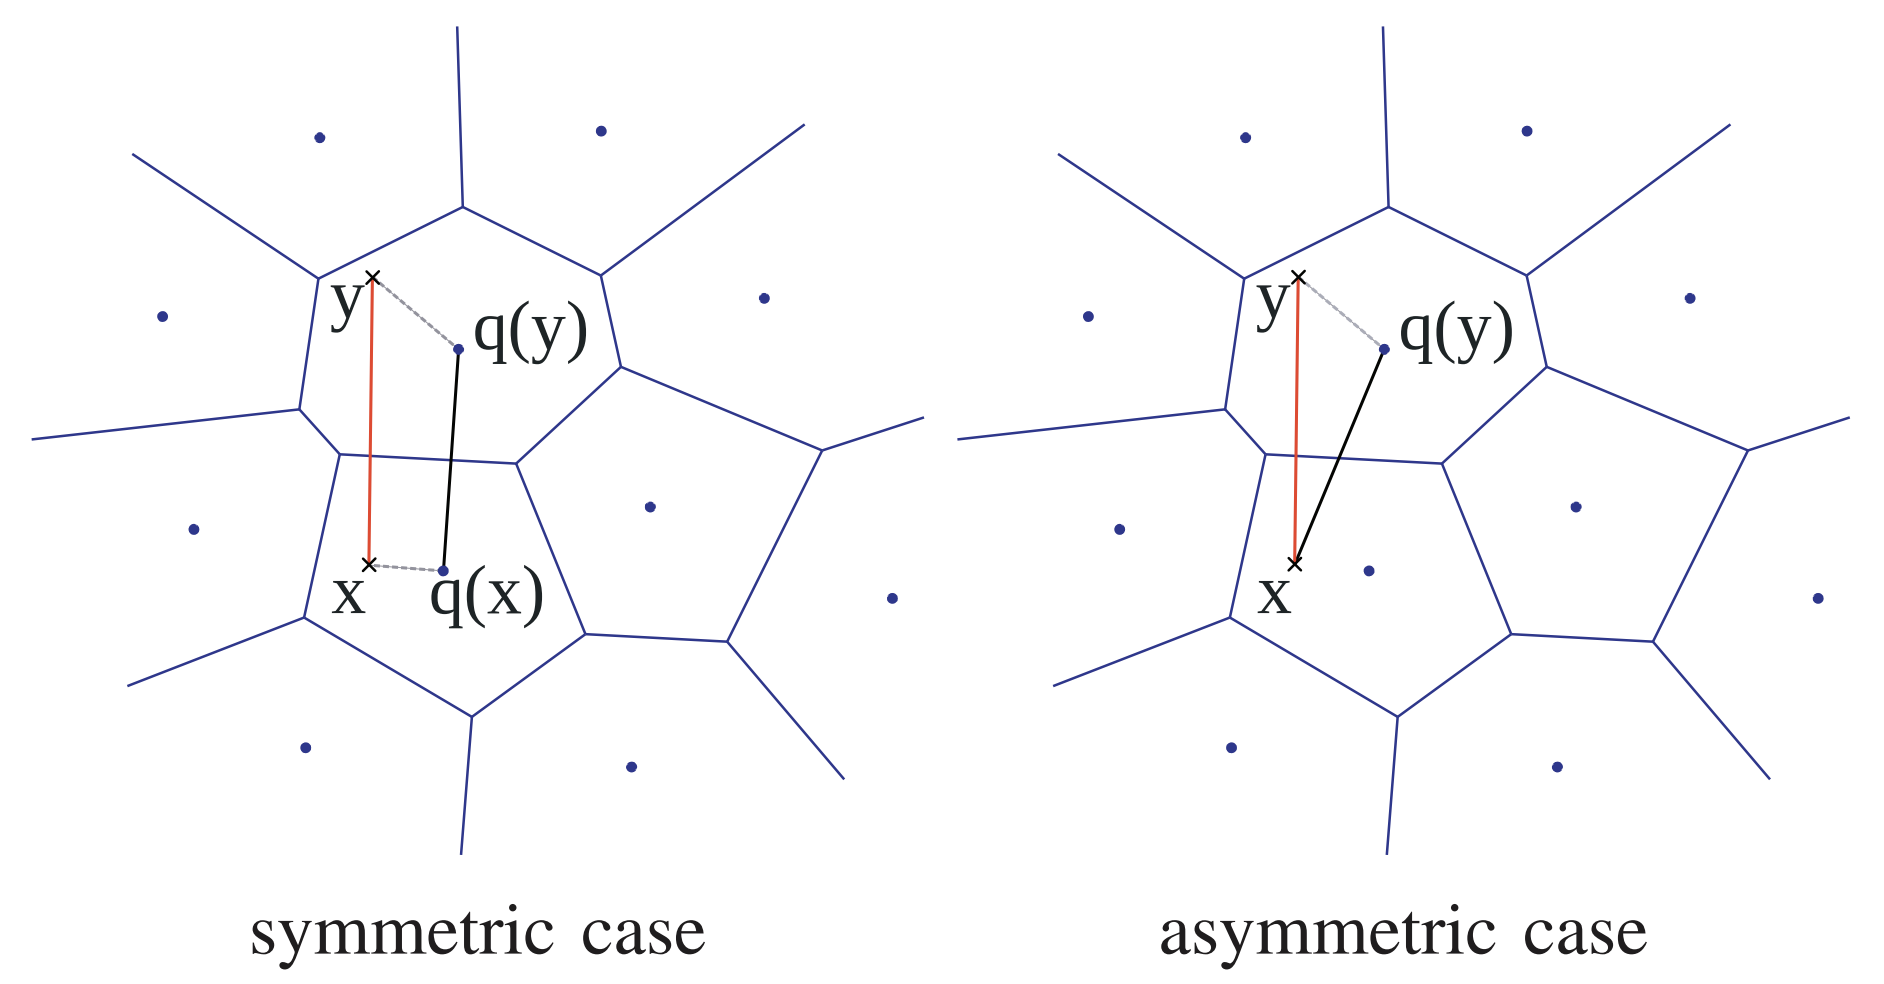
\includegraphics[width=\linewidth]{figures/pq}
\caption{Figure by Jegou et al.~\cite{jegou2010product} illustrating the difference between symmetric and asymmetric estimation, as used in Euclidean Nearest Neighbour Search.
   The distance $q(y)-x$ is a better approximation of $y-x$ than $q(y)-q(x)$.
   In the set setting, when $q$ is MinHash, it is not clear what it would even mean to compute $q(y)-x$?
   %(The voronoi cells are sets that sample to the same minhash value)
}
   \label{fig:jegou}
\end{figure}


While asymmetric estimation is a natural idea for Euclidean distance, it is less clear how it might apply in the context of set search and MinHash quantization.
Somehow we have to compute a similarity value, given $X$ and $q(Y)$ better than $\|q(X)-q(Y)\|_1/K$.
%, since presumably we're throwing information away about $X$ by sketching it.
An indication that this may be possible is the case where the MinHash value of $Y$ is not equal to the MinHash of $X$, but is perhaps equal to the second or third smallest value---that ought to count as evidence towards the sets being similar, even if the classical MinHash sketch would count it as evidence to the opposite.

\subsection{Results}

In this paper we take a principled approach to this problem.
\begin{enumerate}
   \item We derive an estimator based on maximum likelihood.
      We analyse its variance, which we find to be $28\%$ lower than the classical sketch-space estimator.
      (See figures \ref{fig:mle_variance} and \ref{fig:var}.)
      For small similarities the we reduce the variance by a factor $\frac{|Y|}{|X|+|Y|}$ showing particularly good results when the (known) set $X$ is much larger than the unknown set $Y$.
   \item We investigate relaxations and numerical methods, trading precision for speed of estimation. (See tables \ref{tab:netflix} and \ref{tab:flickr}.)
      A particular good choice is dubbed the ``Minner Estimator'' since it is based on counting the number of elements in $X$ that hash to a value \emph{smaller than the minimum} hash value of $Y$.
   \item We run experiments on several large set datasets from~\cite{mann2016empirical},
      such as the Netflix dataset originally from \href{https://www.cs.uic.edu/~liub/Netflix-KDD-Cup-2007.html}{KDD-Cup 2007}.
      We show a reduction in the MinHash values needed of up to 30\% for a given recall@10.
\end{enumerate}

While our focus is mainly on applications characterized as ``one-many'', such as search, many applications characterized as ``many-many'' are trivially reduced to $n$ times one-many.
We thus also obtain better performance for important tasks such as duplicate detection and nearest neighbour graph construction.

% TODO: Go over this one more time
A non-goal of the paper is to make the fastest possible implementation of Set Similarity Search.
For this reason we don't include experiments measuring the runtime of our estimators.
To be competitive in raw running time requires a serious engineering task with papers like~\cite{guo2020accelerating} including 33,812 lines of optimized C and assembly code by many authors.
In \cref{sec:alg} we discuss hardware level optimizations of this kind.

\subsubsection{Lower $K$ for a given Variance and Recall}

% Rasmus: ``Synes at introen er god. Kunne måske være mere eksplicit om hvad det er du måler. Er plads fx i antal bits eller antal elementer? Hvorfor netop varians?''
Technically, the most difficult part is in the precise variance analysis of the maximum likelihood estimator.
Since our estimators are unbiased, the variance corresponds to the mean squared error when estimating similarity for pairs of sets.
A factor two loss in variance would need to be counterbalanced by a factor two increase in the number of MinHash values, significantly reducing practical performance.
One may ask other questions, such as the necessary $K$ to obtain high probability confidence bounds,
but since we work with independent values, this is mostly trivial.

An important ``downstream'' measure is the recall on real datasets.
This determines how large a $K$ is needed in order to return the true nearest neighbour when scanning a database with estimated similarities.
The exact value depends heavily on the ``difficulty'' of the dataset, and varies between 20 and more than 500 for a 90\% recall@10 in our experiments.
In every case our new method is able to obtain a significantly higher recall when given the same information as is available to the classical MinHash estimator.

Other papers have focused on compressing the MinHash sketch itself, a famous algorithm being the~\cite{flajolet2007hyperloglog}.
In general $O(\log\log u + K\log K)$ bits suffice for similarity estimation~\cite{DBLP:reference/algo/Cohen16b}, improving over storing the ranks directly with $\lceil K\log_2 u\rceil$ bits.
Our paper differs by focusing on \emph{reducing $K$}, which can then be combined with those results for even greater compression.
Reducing $K$ also has the benefit of increasing processing speed, something not gained by simply storing the same sketch in less space.
% Why is this more important than things like b-bit minhash?
% Theoretically, this is related to the ``one way communication complexity'' of set similarity.
% In our analysis we focus on minimizing variance (or squared error, since all but one of our estimators are unbiased).

%! TEX root = ../aminhash.tex

\section{Background and Related work}

Estimators for MinHash, other than the ``classic'' one referred to in this paper, have been derived for various purposes.
Cohen~\cite{DBLP:reference/algo/Cohen16b} made improved estimators for graph algorithms,
and Ertl~\cite{DBLP:journals/corr/Ertl17} derived better estimators for Flajolet's HyperLogLog~\cite{flajolet1985probabilistic} variation of MinHash.
%
The extremely successful Mash~\cite{ondov2016mash} software in Bioinformatics works by
a Bayesian estimator of sketch similarity that takes into account the process of `mer'-tokenization that created the data.
However, for the simple task of estimating similarities in the many-one setting, there appears to have been no prior work.

\begin{figure}
\centering
 \begin{tabular}{|r|r| r r r r r|} 
 \hline
     \multicolumn{7}{|c|}{MinHashed Database} \\
 \hline
 id & Size, $n_y$  & $r_1$ & $r_2$ & $r_3$ & \dots & $r_K$ \\
 \hline
 0 & 254 & 4594 & 4439 & 9295 & \dots & 658  \\
 1 & 107 & 66 & 3675 & 457 &     \dots & 6805  \\
 2 & 3322 & 342 & 1173 & 11 &    \dots & 409  \\
 3 & 501 & 9928 & 226 & 603 &    \dots & 2784  \\
  \hline
 \end{tabular}
 \caption{In this example MinHased Database four sets have been quantized into $K$ values each.
    Instead of storing the value of $h:[u]\to[0,1]$ as a real number we have used the equivalent representation of ranks, in which $h$ is a random bijection $h:[u]\to[u]$.
    This allows for more efficient compression of the MinHash values.
 }
 \label{tab:minhash-example}
\end{figure}





\subsection{Quantization and Search}

Since Jegou et al. 2010~\cite{jegou2010product} quantization has been a critical part of fast search data structures.
In particular, the approach of Product Quantization, which sketches vectors in $\R^d$ in a fast, data-sensitive way.
Recently Guo et al.~\cite{guo2020accelerating} broke all records~\cite{aumuller2017ann} for Maximum Inner Product Search (MIPS) and Cosine Similarity, based on a new Product Quantization technique sensitive to those measures.
The secret to these amazing results is the use of Single Instruction, Multiple Data (SIMD) instructions on modern CPUs, which can consume large batches of quantized data per instruction.

In comparison, the landscape for set similarity search is less developed.
Recent theoretical works~\cite{christiani2017set, DBLP:conf/focs/AhleK20} have discovered the optimal randomized space partitions to use and replaced MinHash after 20 years as the best-known approach.
However, the state of the art implementations~\cite{christiani2018scalable} still use MinHash sketching for faster similarity estimation among points in the space region.
In contrast to the Euclidean case, they have thus far had to the classical symmetric estimator.


% Relation to one-way communication complexity.

\subsection{Alternative sketches}

There are a number of other sketches for estimating set similarity that we do not study in this paper.
In general, any sketch that allows cardinality estimation and taking the union of two sketches can be used to estimate the set overlap and similarity.
Most estimators for these sketches are of the symmetric type, so it would be interesting to study whether some of them have good asymmetric estimators as well.

HyperLogLog~\cite{flajolet2007hyperloglog}, HyperMinHash~\cite{yu2020hyperminhash}, MaxLogHash~\cite{wang2019memory}, SetSketch~\cite{DBLP:journals/corr/abs-2101-00314} and $b$-Bit MinHash~\cite{li2010b} focus on compressing coordinated samples, however they don't try to get extra information \emph{per sample} as we do in this paper.

MinHash itself has variations, such as bottom-$k$ MinHash and $k$-partition MinHash.
Cohen~\cite{DBLP:reference/algo/Cohen16b} gives a nice survey of those as well as many more variations and applications.
Thorup~\cite{thorup2013bottom} analyses bottom-$k$ in a setting superficially similar to ours: For two sets $Y\subseteq X$ and $S$ a bottom-$k$ sketch of $X$, he bounds the deviation of $|S\cap Y$ from its expectation.
That is, he compares a sketched set with an unsketched set.
However, since $Y$ is a subset of $X$ it turns out, that for bottom-$k$ the intersection $S\cap Y$ is the same as $S\cap S(Y)$, so he is still in the classical ``symmetric'' setting.

%TKDE 2018 A Review for Weighted MinHash Algorithms
%(How does my method relate to weighted minhash?)


%! TEX root = ../aminhash.tex

\section{The Estimators}

In this section we develop a maximum likelihood estimator (MLE) for MinHash, analyse the variance and compare it to the classical MinHash estimator.
Such an estimator has the lower possible variance asymptotically as $K\to\infty$, but it is slow to evaluate, which destroys the gains from needing fewer MinHash values.
We thus proceed to develop a third estimator that is as fast as the classical estimator.
We call it the Minner estimator and we show experimentally that it requires nearly as few MinHash values as the MLE for equivalent recall.
In fact, for $K < 50$ it requires fewer values than even the MLE.

A quick note on notation: If $u\in\mathbb N$, we use $[u]=\{0,\dots,u-1\}$ to indicate the set of numbers up to $u$.
If $P$ is a proposition, we use $[P]$ to indicate the variable that is $1$ if $P$ and $0$ if not $P$.

\subsection{Maximum Likelihood Estimator}

Given a random variable and a statistical model, ``estimation'' is the task of inferring the parameters to the model on the basis of the observation.
A maximum likelihood estimator chooses the parameters that maximizes the probability that the model generates the particular observed value.
That is, if the observation is equal to $\rho$ with probability $p(\rho;\,\theta)$, $\theta$ is unknown, once we observe $\rho$, we estimate $\theta$ as the $\argmax p(\rho;\,\theta)$.

% A statistical model for a MLE contains four types of variables:
% Those we know at the time of estimation;
% those that are random but we observe;
% those that are random and hidden;
% and those we want to estimate.

In our case we get the following model:
Given a set $X$, a hash function $h:U\to [0,1]$, and values $n_y$ and $v$, we sample a set $Y\subseteq U$ with $|Y|=n_y$ and $v=|X\cap Y|$.
We let $r$ be the smallest value $h(y)$ for $y\in Y$.
The log-likelihood of the observation is then:
\[
   \ell(r; v) = \log\Pr_{Y}[\min_{y\in Y}h(y) = r].
\]
We note a couple of things about the model:
1) By assuming $Y$ is generated uniformly at random among sets of size $n_y$ and overlap $v$ we are making a specific choice that may not be optimal for all datasets.
In the ``skewed data'' model of~\cite{mccauley2018set} a Bayesian might incorporate a particular presumption about the sets $Y$ and increase the precision of the estimator.
2) We can get the same model by taking $Y$ to be known, but the hash values $h(y)$ to be unknown.
This is more similar to the classical MinHash analysis, but doesn't make a big difference in our case, except by making it harder to be a Bayesian.
3) If we do not consider $n_y$ to be known, we can let the model have two parameters and estimate both of them.
We could for example count the frequency of set sizes in the database and build this into the model, however in the database model we might as well just store the set sizes and use them directly.

As a first step to computing $\ell(r;v)$ we not that $h$ can be assumed to take values in $[u]$ rather than $[0,1]$ and a be a bijection.
However then $h$ simply represents a known permutation of $[u]$ and we can ignore it all together.
Then the observed MinHash value is the random variable $R=\min_{y\in Y} y$.
We define $n_x = |X|$, and $M = \sum_{x\in X} [x < R]$ to be the number of ``minner values'' -- a random variable which is a function of $R$.
We proceed to prove the following proposition:
\begin{proposition}
   Let $r\in[u]$ be the MinHash of $Y$ and let $y^*$ (also $\in[i]$) be its index such that $h(y^*)=r$.
   Let $m=m(r)=\sum_{x\in X}[x < r]$ then
\[
   \Pr_Y[R=r]
    =
    \begin{cases}
      \frac{\binom{n_x-m-1}{v-1}\binom{u-r-(n_x-m)}{n_y-v}}{\binom{n_x}{v}\binom{u-n_x}{n_y-v}}
      &
      \text{if $y^*\in X$, and}
       \\
      \frac{\binom{n_x-m}{v}\binom{u-r-1-(n_x-m)}{n_y-v-1}}{\binom{n_x}{v}\binom{u-n_x}{n_y-v}}
      & \text{if $y^*\not\in X$}
    \end{cases}
 \]
 \label{prop:prob}
\vspace{-1em} %Some weird spacing going on here.
\end{proposition}
Note we take $\binom{n}{k}=0$ for $n<k$.
In particular this may happen if $n_x-m<v$.
The probability of $R=r$ in this case is 0, since $n_x-m$ is the number of x-ranks at least $r$, and all of $X\cap Y$ must have rank at least $r$.
\begin{proof}
   Not considering $R$ there are $\binom{n_x}{v}\binom{u-n_x}{n_y-v}$ ways to choose $Y$ such that $|Y|=n_y$ and $|X\cap Y|=v$.
   We proceed by cases..

   First consider the case $r\in X$.
   Then the remaining $v-1$ overlapping elements have to be chosen from $\{x\in X:x > r\}$.
   by definition of $m$ there are $n_x-m-1$ such values.
   The remaining $n_y-v$ non-overlapping elements have to be chosen from $\{x\not\in X: x > r \}$.
   There are $u-r$ elements in $[u]$ greater than $r$, and of those $n_x-m$ are in $X$.
   Thus the number of ways to choose $Y$ with $r\in X$ is
   $\binom{n_x-m-1}{v-1}\binom{u-r-(n_x-m)}{n_y-v}$.

   The case $r\not\in X$ follows by similar arguments.
\end{proof}

Using \cref{prop:prob} we can write the log-likelihood in the following concise manner:
\[
   \ell(r; v) = \log \frac{\binom{n_x-m-[r\in X]}{v-[r\in X]}\binom{u-r-[r\not\in X]-(n_x-m)}{n_y-v-[r\not\in X]}}{\binom{n_x}{v}\binom{u-n_x}{n_y-v}}.
   \label{eq:log-likelihood}
\]
If we observe $K>1$ values $r_1, r_2, \dots, r_K$ we get, by independence of the MinHash functions, a log likelihood of
\[
   \ell(r_1; v) + \ell(r_2; v) + \dots + \ell(r_K; v).
\]
It is trivial to enumerate all $v\in[\min\{n_x,n_y\}+1]$ and compute which one has the highest log-likelihood.
\begin{definition}[Maximum Likelihood Estimator (MLE)]
   The maximum likelihood estimators for respectively set overlap and Jaccard similarity are
   \begin{align}
      T_v(r_1,\dots,r_K) &= \argmax_{v\in[\min\{n_x,n_y\}+1]} \ell(r_1; v) + \ell(r_2; v) + \dots + \ell(r_K; v).
      \\T_j(r_1,\dots,r_K) &= \frac{T_v(r_1,\dots,r_K)}{n_x+n_y - T_v(r_1,\dots,r_K)}.
   \end{align}
\end{definition}
%
The definition gives our first estimator.

\subsection{Analysis}

We want to analyse the MLE estimator in the model where $h$ is unknown.
In this setting we know that the variance of the classical MinHash estimator is
\[
   \frac{E[(T-j)^2]}{K}
      = \frac{E[T^2] - j^2}{K}
      = \frac{\Pr[T=1] - j^2}{K}
      = \frac{j(1-j)}{K}.
      \label{eq:minvar}
\]
This is important because we want to know the general expected performance of the algorithm, and not what it does after some particular random event.

TODO: We should talk about bias before variance.

The main work of this section will be proving the following proportion:
\begin{proposition}\label{prop:mle_var}
   As $K\to\infty$, the variance of the MLE estimator converges to
   \[
      \frac{j (1+j)^3 n_y (n_y-j n_x) (n_x-j n_y)}{(n_x+n_y) \left((1+j)^2 n_xn_y - j^2 (n_x+n_y)^2\right)K}
   \label{eq:mle_var}
   \]
   over the randomness of the random hash function.
\end{proposition}

\begin{figure}
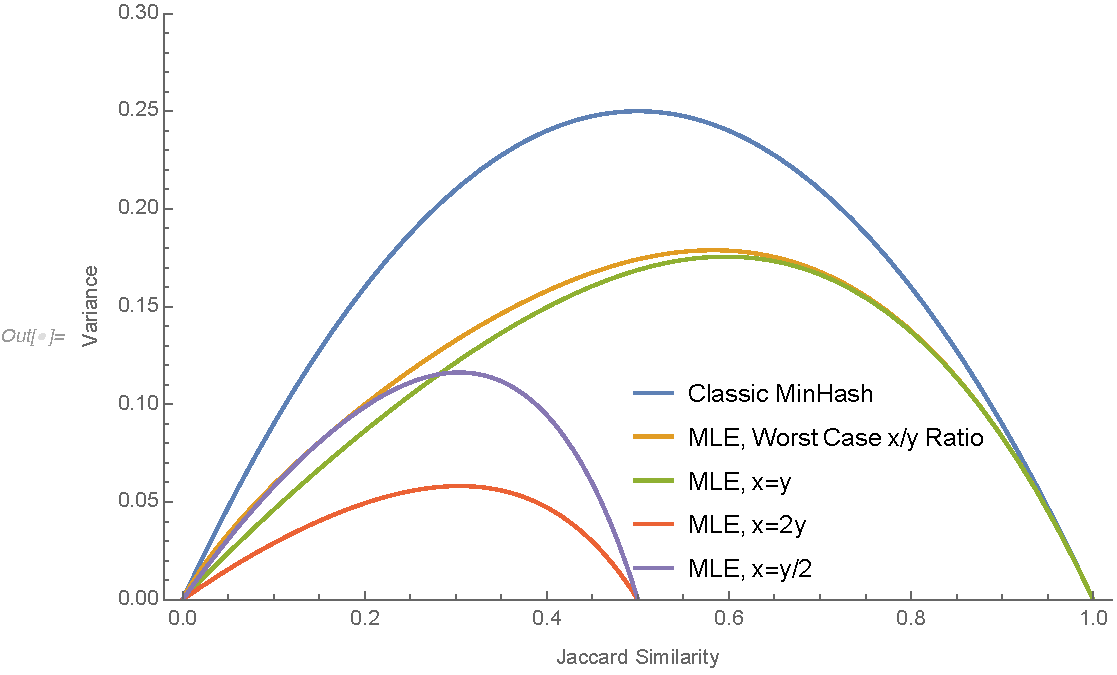
\includegraphics[trim=30 0 0 0,clip,width=\linewidth]{figures/mle_variance2}
\caption{Variance of maximum likelihood estimator based on Fischer Information bound.
For $j$ close to 0 or 1 the worst case MLE bound is asymptotically equal to the Classical bound, whereas for $j\approx 0.21$ has only $\approx 62\%$ of the variance.
See \cref{fig:exp_variance} for a corresponding experimental test.
}
\label{fig:mle_variance}
\end{figure}

The bound is a little complicated by the fact that it includes the sizes of the sets $n_x$ and $n_y$.
We note that the bound is convex in the ratio $n_y/n_x$, giving lower variances than \cref{eq:minvar} for $n_x<\!<n_y$ or $n_x >\!> n_y$.
\Cref{fig:mle_variance} shows \cref{eq:mle_var} when the ratio is taken to be \emph{worst possible}, as well as when it is taken to be 1
In the symmetric case $n_x=n_y$ the asymptotic variance reduces to
\[
   \frac{j(1-j)}{K}\frac{(1+j)^3}{2(1+3j)}.
\]
%for large $x$ and $y$.
For $n_x/n_y\neq1$ the Jaccard similarity is bounded above by $\frac{\min\{n_x,n_y\}}{\max\{n_x,n_y\}}$, which allows the MLE to discard those higher values from consideration.
Another interesting point from \cref{eq:mle_var} is that the variance at $n_x=c n_y$ is exactly $1/c$ of the variance at $n_x=n_y/c$.
It makes sense that the variance is lower when $|X|$ is big compared to $|Y|$, since we are given $X$, but don't know $Y$.

TODO: Stuff about local/global risk.
We can also compute the global risk of the MLE estimator, which is $0.178847/K$, $28.5\%$ less than the Classical Estimator.

\begin{proof}[Proof of \cref{prop:mle_var}]
   We first find the variance for the MLE estimator for $v$ and then show how to re-parametrize it to use the Jaccard similarity.

   Using Stirling's approximation $ \log n! = n\log n - n + O(\log n)$,
   we rewrite the log-likelihood \cref{eq:log-likelihood} as
   \begin{align}
      \ell(r;v) &=
      (x-k-[y^*\in X]+1)H(\tfrac{v-[y^*\in X]}{x-k-[y^*\in X]+1})
               - (x+1) H(\tfrac{v}{x+1})
              \\&+(u-m-[y^*\not\in X]-x+k+1) H(\tfrac{y-v-[y^*\not\in X]}{u-m-[y^*\not\in X]-x+k+1})
              \\& -(u-x+1) H(\tfrac{y-v}{u-x+1})
   + O(\log u),
   % TODO: We should probably also have error terms for n_y-v, n_x-v and so on.
   \end{align}
   where $H(p)=p \log \frac{1}{p} + (1-p)\log \frac{1}{1-p}$ is entropy function.

   Standard results~\cite{panchenko2016lec3} on maximum likelihood estimators say that
   the variance converges to $1/I(v)$ where
   \[
      I(v) = E\left[-\frac{d^2}{dv^2}\ell(m;v)\right]
   \]
   is known as the Fischer information.
   \footnote{This is actually a bit more tricky than it seems, since
      the standard proof of this fact~\cite{panchenko2016lec3} uses that the expectation is taken over the same probability space as $\ell$ is defined.
      However one can check that the key step in which that is used is to show
      $E[f''/f] = \int (f''(x)/f(x))f(x)dx = \int f''(dx) = (\int f(x)dx)'' = 0$, where $f=\exp(\ell)$ is the probability distribution.
      Since $E_h[f''/f] = E_h[E_{h_{|\overline X}}f''/f] = E_h[0]= 0$
      we can run the entire proof using $E_h$ rather than $E_{h_{|\overline X}}$ and get the same result.
      Thus it suffices to thus focus on bounding $E_h[-\frac{d^2}{dv^2}\ell(m;v)]$.
   % Something, something sigma algerba.
      % Basically I'm arguing that we can run the whole proof of MLE asymptotics and consider very expectatation as over $E_h$ rather than $E_{h_{|X}}$
   }

   % Strictly speaking the Fischer information is only defined when the log-likelihood is differentiable in the parameter $j$, which is not the case here, since we know $\frac{j}{1+j}(x+y)$ is an integer.
   %Since Stirling's approximation also applies to derivatives (simply exchanging the sum and the derivative operator)

   TODO: Update notation
   We can now evaluate the first two derivatives:
   {
      \thinmuskip=0mu
      \begin{align}
         % Single diff
         \frac{d}{dv}\ell(m;v)
         &=
         \log\left(\frac{(1-\frac1{y-v+1})^{[y^*\not\in X]}(1-\frac{k}{x-v+1})}{(1-\frac 1{v+1})^{[y^*\in X]}(1-\frac{m-k}{u-x-y+v+1})}\right) + O(1/u)
         \label{eq:deriv1}
         \\
         % Double diff
         \frac{d^2}{dv^2}\ell(m;v)
        &=
          [y^*\not\in X](\tfrac1{y-v+1}-\tfrac1{y-v})
         + (\tfrac1{x-v+1}-\tfrac1{x-v-k+1})
      \\&+[y^*\in X](\tfrac1{v+1}-\tfrac1{v})
         + (\tfrac1{u-x-y+v+1}-\tfrac1{u-x-y+v-m+k+1})
      \\&+ O(1/u^2)
         \label{eq:deriv2}
         .
      \end{align}
      \vspace{-1em}
   }

   We now have three terms to bound:
   $E[y^* \in X]$, $\tfrac1{x-v-k+1}$ and $\tfrac1{u-x-y+v-m+k+1}$.
   Since any element of $Y$ has even chance of becoming the smallest, we have 
   \[E[y^*\in X] = \Pr[y^*\in X] = \frac{v}{n_y}. \]

   When considering the rank, $r$, and the minner count, $m$, we'll assume the values of $h$ have exponential distribution.
   This corresponds to using $\log1/h(x)$ instead of $h(x)$ which is a strictly monotone transformation and so equivalent in terms of comparing hash values.
   Let $h^* = h(y^*)$ (different from $r$ which is the rank.)
   Then $h^* = \min_{z\in y}h(z) \sim \text{Exp}(y)$ by stability of minimums of exponentially distributed random variables.

   We can now see $m=\sum_{x\in X\setminus Y} [h(x) < h^*]$ as having binomial distribution $B(n_x-v, p)$, conditioning on $h^*$, where $p=\Pr[h(x)\le h^*] = 1-\exp(-h^*)$ by the CDF for the exponential distribution.
   We only sum over $X\setminus Y$ rather than all of $X$ since no value in $X\cap Y$ can be smaller than $h^*$ by definition.
   Because of the binomial revision
   $\frac1{n-i+1}\binom{n}{i} = \frac1{n+1}\binom{n+1}{i}$
   we can evaluate
   \begin{align}
      E_m\left[\tfrac1{n_x-v-m+1}\right]
      &= E_{h^*}\left[\tfrac{1-p^{n_x-v+1}}{(1-p)(n_x-v+1)}\right]
    \\&= \tfrac1{n_y-1}\left(\tfrac{n_y}{n_x-v+1} - \tfrac1{\binom{n_x+n_y-v}{n_y}}\right),
    % TODO: Does something weird happen if v=n_x or v=n_y?
   \end{align}
   where the second equality follows by properties of the exponential distribution.
   Note that the expectation is defined for all $n_y\ge 0$ by limits.%
   \footnote{In particular at $y=1$ it equals $H_{n_x-v+1}/(n_x-v+1)$, where $H_n$ is the harmonic number.}

   We can similar note that $r-m$ is the number of values in the complement of $X\cup Y$, and so has binomial distribution $B(u-n_x-n_y+v, p)$.
   By the same arguments as above, we get that
   \[
      E\left[\tfrac1{u-n_x-n_y-v-(r-m)+1}\right]
      = \tfrac1{n_y-1}\left(\tfrac{n_y}{u-n_x-n_y+v+1} - \tfrac1{\binom{u-n_x-n_y+v}{y}}\right).
   \]
   Combining all the terms of \cref{eq:deriv2}, and assuming $n_x$ and $n_y$ sufficiently large we get the simple result
   \[
   I(v)
   = \frac{1}{n_y(n_x-v)} + \frac1{v(n_y-v)} + O\left( \frac{1}{\min\{n_x,n_y\}} \right).
   \]
   We can now use the re-parametrization formula for Fischer Information to compute
   \[
      %I_j(j) = j'(v(j))^{-2}I_v(v(j))
      I_j(j) = v'(j)^{2}I_v(v(j)),
   \]
   %where $j(v) = v/(x-y+v)$.
   where $v(j) = \frac{j}{1+j}(x+y)$.
   % eta = psi(theta)
   % j = j(v)
   % theta = psi^{-1}(eta)
   % v = j^{-1}(j)
   % I(j) = I(v)
   By the previously stated facts on maximum likelihood estimators, this proves the proposition.
\end{proof}

We have succeeded in analysing the variance of the maximum likelihood estimator.
There are more questions to ask, such as how large $K$ must be to start seeing convergence to the stated bound.
We give some experimental evidence for these questions in \cref{sec:estimation}.

\subsection{Minner Estimator}

\begin{figure}
   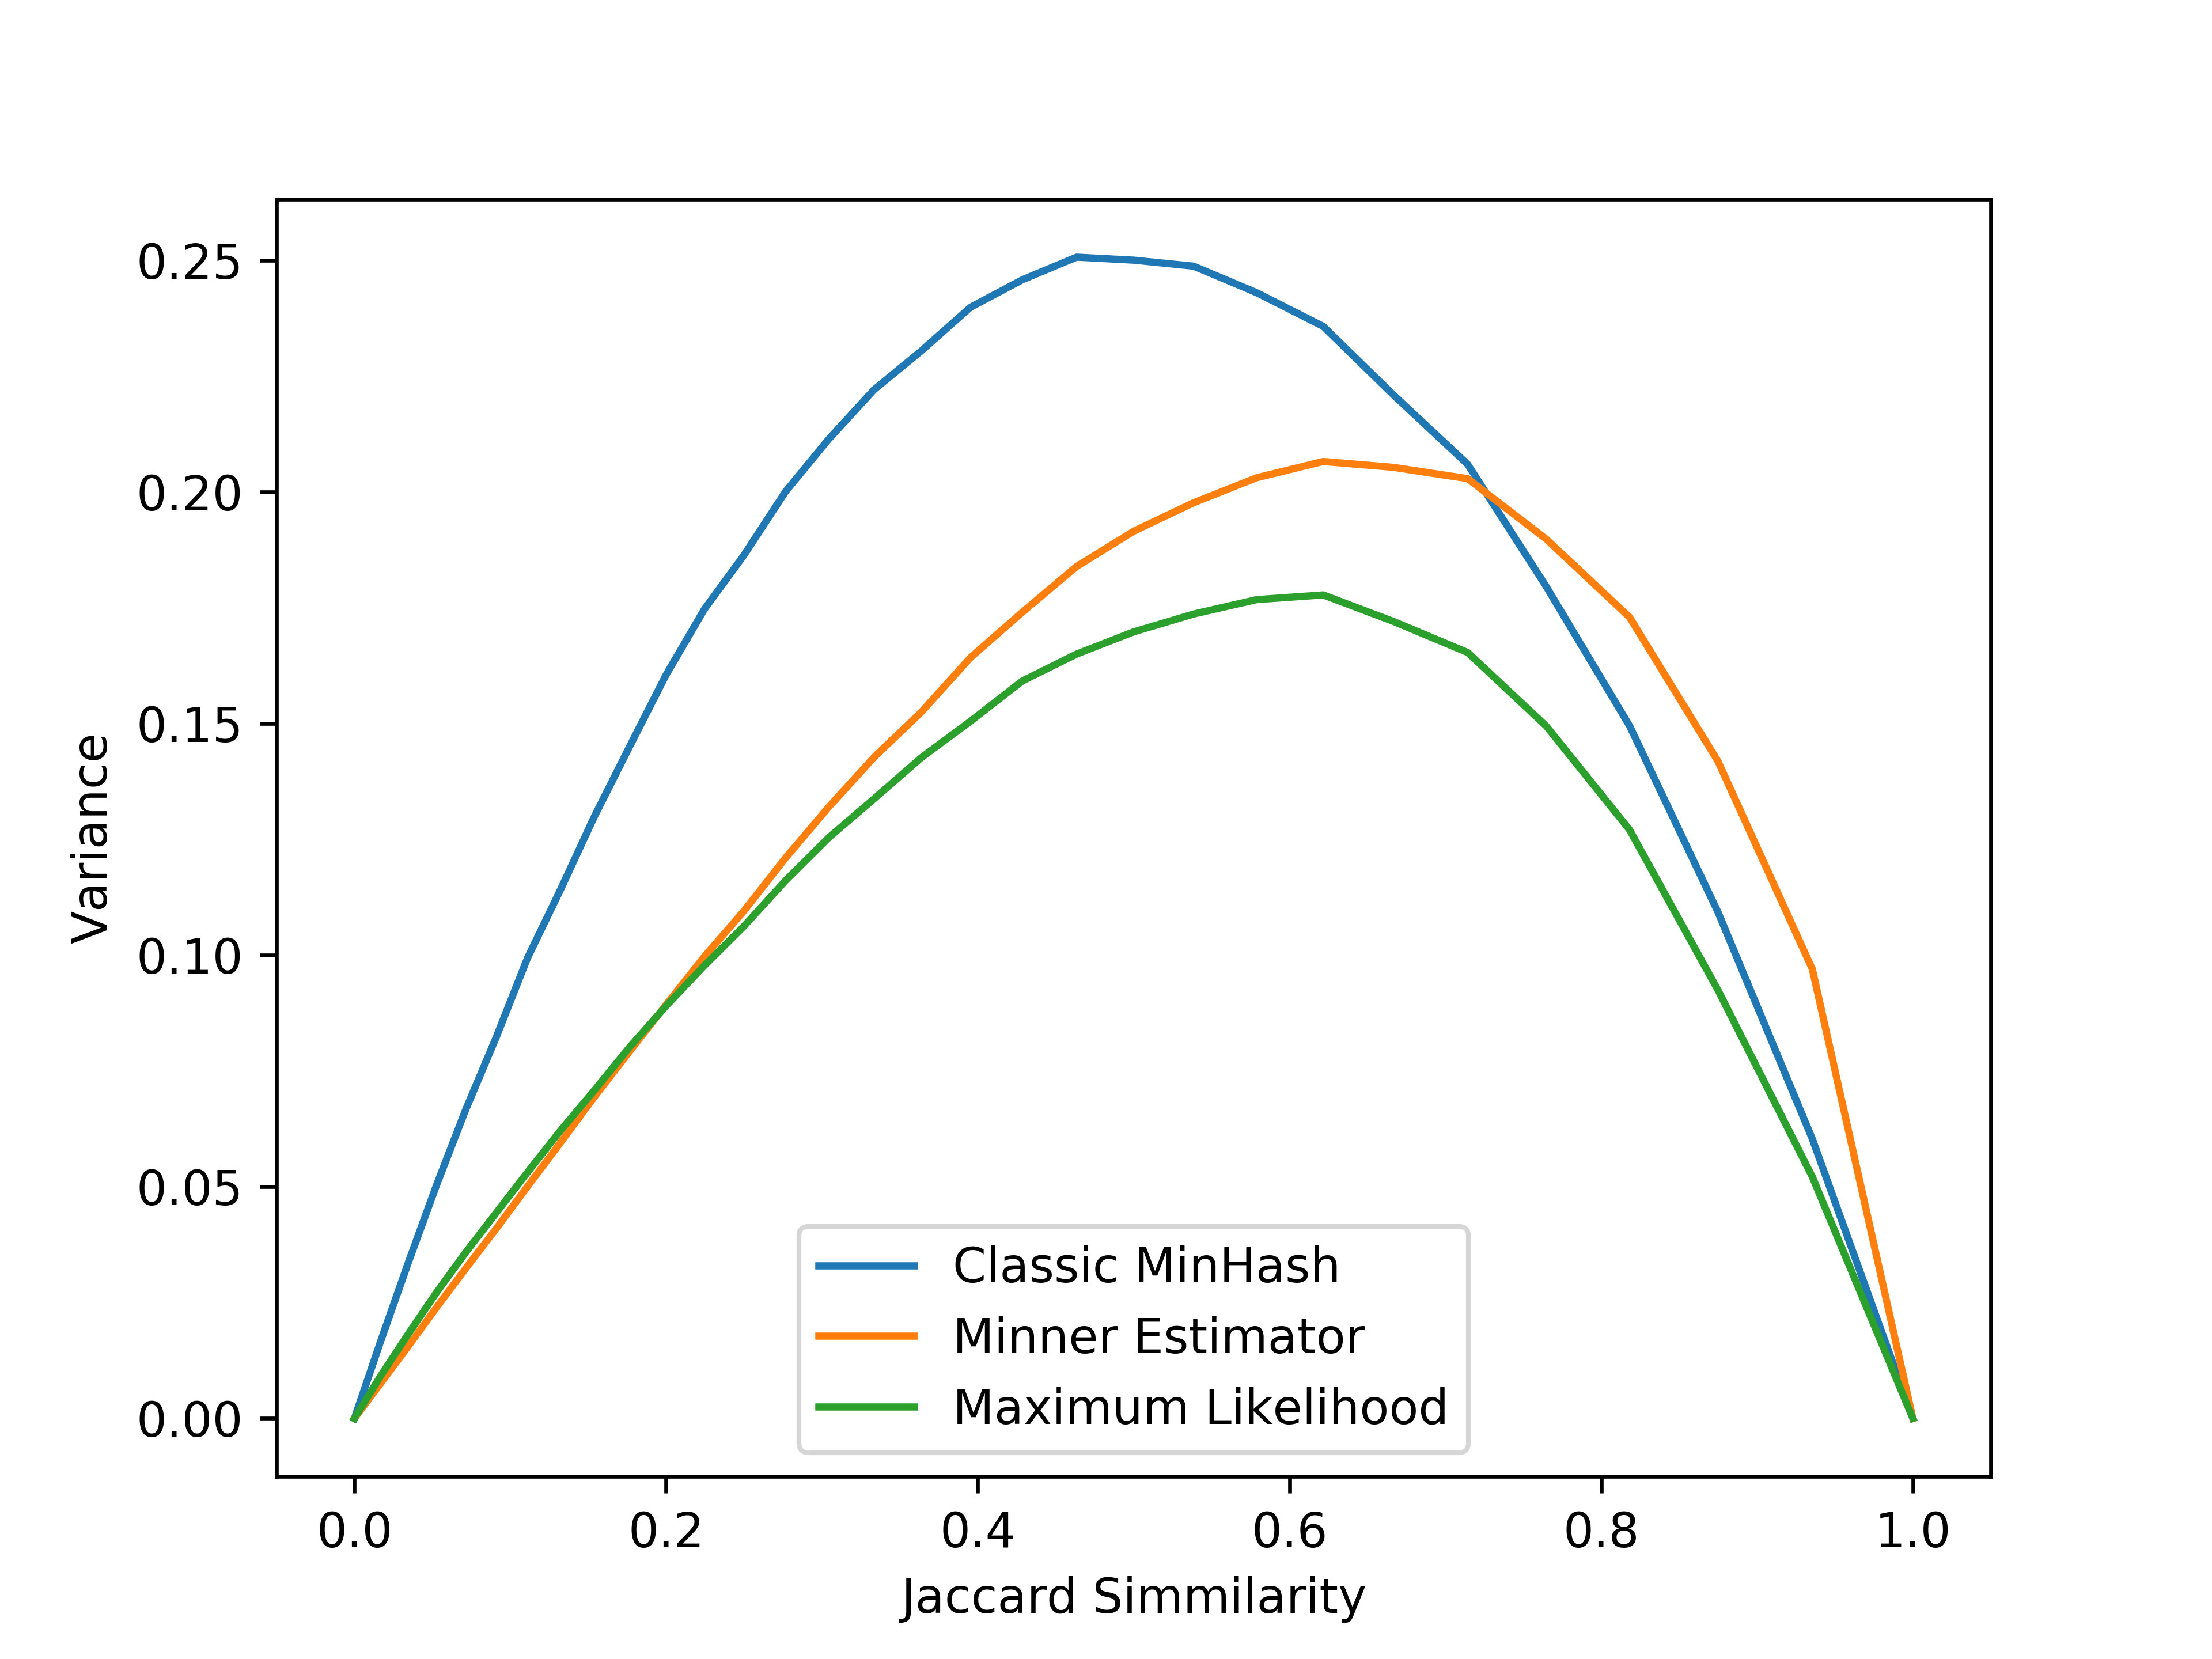
\includegraphics[trim=10 0 45 40,clip,width=\linewidth]{figures/synvar_100000.png}
   \caption{Measured variance of estimators, over 100,000 repetitions at $|X|=|Y|=K=30$ and $u=500$.
      The MLE has already almost converged to \cref{fig:mle_variance}.
      The Minner Estimator is seen to be particular good for low Jaccard similarities, which may be why it works so well on the practical datasets tested in \cref{sec:evaluation} which tend to have similarities concentrated in the $[0,0.2]$ range, as seen in \cref{fig:scatter}.}
   \label{fig:exp_variance}
\end{figure}

In the previous sections we derived and analysed a Jaccard similarity estimator based on maximum likelihood.
The estimator has to evaluate the log-likelihood function, $\ell$, for all $v\in[\min\{n_x,n_y\}+1]$, which means it takes time at least $\Omega(K\min\{n_x,n_y\})$ per database point.

In this section we investigate numerical methods for speeding up the MLE and suggests a new, very fast, estimator we call the Minner Estimator, which can be computed as fast as the classical MinHash estimator.

The starting point of this derivation is the continuous derivative log-likelihood \cref{eq:deriv1},
which we would like to solve $=0$ for $v$.
If we apply the approximation $\log(1-\eps) \approx -\eps$,
we we get
\[
   \frac{d}{dv}\ell(r;v) \approx
   -\frac{[y^*\not\in X]}{n_y-v} 
   -\frac{m}{n_x-v} 
   +\frac{[y^*\in X]}{v} 
   +\frac{r-m}{u-n_x-n_y+v} 
   %= 0
   .
\]
This is a convenient form, since it is linear in the variables, $[y^*\in X]$, $m$ and $r$.
As we observe multiply $r_i$ values, we can define
$R = \sum_i r_i$, $M = \sum_i m_i$ and $C = \sum_i [y_i^*\in X]$.
This gives us a single equation to solve
\[
   \sum_i\frac{d}{dv}\ell(r_i; v) \approx
   -\frac{K-C}{n_y-v} 
   -\frac{M}{n_x-v} 
   +\frac{C}{v} 
   +\frac{R-M}{u-n_x-n_y+v} 
   = 0
   .
   \label{eq:d1_simple}
\]
This equation can be rewritten as a degree three polynomial and solved by standard methods.
The time complexity has thus been decreased from $\Omega(K\min\{n_x,n_y\})$ to $O(K)$ plus the time it takes to find the polynomial roots.

However, solving a polynomial for every point in the database is hardly as fast as the classical MinHash estimator.

However, we would like a simpler estimator still.
In practice $u$ is very large (otherwise it wouldn't be set data), so we'll approximate $\frac{R-M}{u-n_x-n_y+v}\approx 0$.
If we assume $n_y>\!>v$ we may approximate $\frac{K-C}{n_y-v}\approx 0$ we get the simple solution to \cref{eq:d1_simple}, $v=\frac{C n_x}{C+M}$.
Alternatively, if $n_x>\!>v$ we approximate $\frac{M}{n_x-v}\approx 0$, we get $v=\frac{C n_y}{K}$.
We then combine the two approximations into the following estimator:
\begin{definition}[Minner Estimator]
\[
   T_v(r) = \min\left\{\frac{C n_x}{C+M}, \frac{C n_y}{K}\right\}.
   \label{eq:minner}
\]
\end{definition}

The resulting value is clearly always in the acceptable range $[0,\min\{n_x, n_y\}]$, since $C\le C+M$ and $C \le K$.
To estimate Jaccard we take $T_j(r) = v/(n_x + n_y - v)$.
As before we can compute $C$ and $M$ in $O(K)$ time per database point, and now we have replaced the finalization of finding the roots of a polynomial with a simple division.

\hspace{.2em}

While $E[\frac{C n_y}{K}] = v$ is nice and unbiased (for estimating $v$), the combined estimator is not necessary so.
Using the arguments from the previous analysis section, we find that for a single observation,\footnote{We were not able to analyse the case where $C$ and $M$ are the sum of multiple $c_i$ and $m_i$ values, nor the effect of combining the two estimators using the minimum.}
\begin{align}
   E[\frac{c n_x}{c+m}]
   &= \frac{v n_x}{y} E[\frac{1}{1+m}]
   = \frac{v n_x}{n_x-v+1} (H_{n_x+n_y-v} - H_{n_y-1})
 \\&\approx \frac{v n_x}{n_x-v+1} \log\frac{n_x+n_y-v}{n_y-1},
 \label{eq:minner_mean}
\end{align}
where $H_n$ is the $n$th Harmonic Number.
If we let $n_x=n_y=n\to \infty$ we get $\eqref{eq:minner_mean} = \frac{2j}{1-j}\log\frac{2}{1+j}$, a quantity sandwiched between the Jaccard similarity, $j$, and the Sørensen–Dice coefficient, $\frac{2j}{1+j}$.
While not unbiased, this is at least monotone in $j$ (respectively $v$).

Experimentally, the actual Minner Estimator seems to converge to $j$ for larger $K$, at least for the smaller $j$ seen in practice. See~\cref{fig:var}.
For larger Jaccard similarities it slightly underestimate them, just as we see on the variance get worse as $j\to1$ in~\cref{fig:exp_variance}.

\hspace{.2em}

We finally present a numerical way to combine the speed of the Minner Estimator with the consistency of the MLE.
The idea is a common one in MLE design, which is to apply Newton's method to the problem of solving $\frac{d}{dv}\ell(r;v)=0$.%
\footnote{People sometimes use Newton's method with the expected Hessian instead of the actual second derivative~\cite{longford1987fast}, however in our case we'll be able to efficiently compute it exact.}
To maintain $O(K)$ complexity per database point we apply Newton's method to the approximate derivative equation \cref{eq:d1_simple}.
This is nice, because the second derivative is still linear in $C$, $R$ and $M$:
\[
   \sum_i\frac{d^2}{dv^2}\ell(r_i; v) \approx
   \frac{K-C}{(n_y-v)^2} 
   +\frac{M}{(n_x-v)^2} 
   +\frac{C}{v^2}
   +\frac{R-M}{(u-n_x-n_y+v)^2}
   .
   \label{eq:d2_simple}
\]
Newton's method now proceeds with iterations
$v_{i+1} = v_i - \frac{\ell'(r; v_i)}{\ell''(r; v_i)}$.

This concludes the derivation of the Minner Estimator with Newton refinement.
In the next section we give pseudo-code matching what was used to perform our experiments on real world data.


%! TEX root = ../aminhash.tex

\section{Implementation Details}

While the algorithm is simple conceptually, there are a few tricks to making it run as fast as the classical MinHash sketch.\footnote{We don't strive to be faster than the classical estimator for a fixed $K$, but for a given recall we can be faster, since our $K$ can be smaller.}

\begin{algorithm}[H]
   \caption{Given a query $X\subseteq [u]$ and a database $D\in [0,1]^{n\times K}$ of sketches of sets $Y_1,\dots\subseteq [u]$, the algorithm estimates the similarity with each $Y_i$.}
   \label{alg:query}
   \begin{algorithmic}[1]
      \For{$j=1$ to $K$}
         \State $H_j \gets \text{sorted}(\{h_j(x) : x \in X\})$
      \EndFor
      \State Initialize a max-heap.
      \For{$i=1$ to $n$}
         %\Comment{Number of contained values, minner values and sum of hashes.}
         \State $C, M, V \gets 0, 0, 0$
         \For{$i=1$ to $K$}
         \State $V \gets V + D_{i,j}$
            \State $C\gets C + [D_{i,j} \in H_j]$ \label{line:contains}
            \State $M \gets M + \sum_{v\in H_j} [v < D_{i,j}]$ \label{line:prefix}
         \EndFor
         \State $y \gets |Y_i|$
         \State $v \gets \min\{\frac{C|X|}{C+M},\frac{Cy}{K}\}$
         \Comment{Minner Estimator}
         \For{$i=1$ to Newtons}
            \State $\nu \gets \frac{V/u + C/(v+1) - (K-C)/(y-v+1) - M/(|X|-v+1)}
            {C/(v+1)^2 + (K-C)/(y-v+1)^2 + M/(|X|-v+1)^2}$
            \State $v \gets \min\{\max\{0,v\}, |X|, y\}$
         \EndFor
         \State $j \gets v/(|X| + y - v)$ \Comment{If Jaccard similarity is required.}
         \State Push $(j,i)$ to the max-heap if big enough.
      \EndFor
   \end{algorithmic}
\end{algorithm}

In \cref{alg:query} we show how one may use our estimator to do a fast scan through a database.
We assume $D_{i,j}\in[0,1]$ stores the minimum hash value of $Y_i$ under hash function $h_j$.
It is perhaps more typical to have $D_{i,j}$ store the $\argmin_{y\in Y_i}h(y)$, but in that case one can simply compute $h(D_{i,j})$ at runtime, which is usually a very cheap function.
The MinHash survey of Cohen~\cite{DBLP:reference/algo/Cohen16b} discusses many very efficient ways of storing MinHash values.

In \cref{alg:query} we start by hashing each element of $X$ under the $K$ hash functions.
We sort the resulting values, to be able to perform \cref{line:contains} and \cref{line:prefix} more efficiently.
These lines respectively check if a given $Y$ hash-value is also in $X$, and counts how many hash-values from $X$ are smaller than the $Y$ hash-value.

There are many ways to perform these tasks.
If the range of $h$ is small, say under a million, we can precompute tables.
For large ranges, we can use that the $H_j$'s are sorted and binary search, which works for both tasks.
In practice, if $|Y|$ is not too much bigger than $|X|$, a linear scan of $H_j$, will yield the right position in constant time.
One can also use one of a plethora of fast prefix sum data structures, which are particularly simple since the values of $H_j$ are uniformly random.
% TODO: Mention that thing about makeing |X| buckets and precomputing the prefix sums?

%! TEX root = ../aminhash.tex

\section{Evaluation by Experimentation}\label{sec:evaluation}

In this section, we show our proposed estimators lead to improved performance on maximum
Jaccard similarity search on real datasets.

First, we fix the quantization
mechanism and compare traditional reconstruction
loss with our proposed loss to show that score-aware
loss leads to better retrieval performance and more accurate estimation of maximum inner product values.
Next, we compare in fixed-bit-rate settings against
QUIPS and LSQ, which are the current state-of-the art for many MIPS tasks. Finally, we analyze the
end-to-end MIPS retrieval performance of our algorithm in terms of its speed-recall trade-off in a
standardized hardware environment. We used the
benchmark setup from ann-benchmarks.com, which
provides 11 competitive baselines with pre-tuned parameters. We plot each algorithm’s speed-recall curve
and show ours achieves the state-of-the-art.

Something about how we can do regression on the tables and get a number of tables saved as a function of required recall.
We assume a simple model $r = 1-\exp(-aK+b)$

\subsection{Recall vs Memory usage}

We focus on the measure recall@10, which means how often the estimated top 10 most similar sets contain the true most similar set.
If the searcher wants to obtain the true nearest set, they can use the estimation as a fast first scan over the data, and then compute the true similarities between the query and the 10 candidates.

We are interested in how the number of hash functions / hash values per stored set trades with the recall.
The number of such values is directly proportional to the memory required to store the dataset.
%We measure memory in the number of independent hash functions we need to store values from.
\footnote{Each value can be stored in a word, and it is possible to compress them further, usually down to around a byte without loss of accuracy.}

The following shows the effect on recall@10 with 10,000 queries:

These results use the minhash estimator as the initial guess.
An alternative is to estimate $v$ as $by/K$, since $Eb=v/y$.
However that appears to be worse, giving recall 1@10 of 0.1718 at newton=1 and $K=30$.
With more newton steps, however, the recall "recovers" to 0.1889 at newton=8.
($n=2$ and $n=4$ gives recall 0.1754 and 0.1826 respectively.)

%Some timing data:
%Tid for -K 100 --newton 1
%Time preparing: t1=2813.205824613571, Time searching: t2=5754.812134742737
%Tid for -K 100 --newton 2
%Time preparing: t1=2768.65847158432, Time searching: t2=5648.562669038773
%Tid for -K 100 --newton 4
%Time preparing: t1=2715.9863698482513, Time searching: t2=5616.8901562690735
%Tid for -K 100 --newton 8
%Time preparing: t1=2769.066630601883, Time searching: t2=6230.902306318283
%
%-K 1 --newton 8
%Time preparing: t1=31.681596994400024, Time searching: t2=765.3667838573456

The first table was wrong, because it didn't account for points with equal similarity.
The following table fixes that problem:
\begin{table}
\centering
 \begin{tabular}{|r| r r r r r|} 
 \hline
     \multicolumn{6}{|c|}{Recall@10 on the Netflix dataset} \\
 \hline
 K  & Classic & MLE & Minner & Minner 1N & Minner 8N \\
 \hline
    1 & 0.0033 & 0.0076 & \textbf{ 0.0099} & 0.0057 & 0.0063 \\
  10 & 0.0501 & 0.0396 & \textbf{ 0.0623} & 0.0506 & 0.0462 \\
  30 & 0.1474 & 0.1773 & \textbf{ 0.1914} & 0.1910 & 0.1862 \\
 100 & 0.3831 &      . & 0.4640 & 0.4870 & \textbf{ 0.4903} \\
 400 & 0.7510 &      . & 0.8054 & 0.8326 & \textbf{ 0.8338} \\
 500 & 0.7942 &      . & 0.8440 & 0.8660 & \textbf{ 0.8667} \\
  \hline
 \end{tabular}
 \caption{The Minner estimator is best at small $K$, but eventually the asymptotics kick in and the Maximum likelihood estimator overtakes. The MLE is very slow however, and one can get most of the benefits by applying a single iteration of Newton's method on top of the Minner Estimator.
    For the midrange $K$ values 30 and 100 we get a near 30\% improvement in recall over the classical estimator.
 }
 \label{tab:netflix}
\end{table}

We can also test on the Flickr Dataset
\begin{table}
\centering
 \begin{tabular}{|r| r r r r r|} 
 \hline
     \multicolumn{6}{|c|}{Recall@10 on the Flickr dataset} \\
 \hline
 K  & Classic & MLE & Minner & Minner 1N & Minner 8N \\
 \hline
    1 & 0.2379 & 0.3410 & \textbf{ 0.3595} & 0.2806 & 0.2969 \\
   5 & 0.6256 & 0.5457 & \textbf{ 0.6688} & 0.5913 & 0.6138 \\
  10 & 0.7770 & 0.7155 & \textbf{ 0.8122} & 0.7327 & 0.7469 \\
  20 & 0.8657 & 0.8540 & \textbf{ 0.8963} & 0.8217 & 0.8352 \\
  30 & 0.9108 & 0.9080 & \textbf{ 0.9301} & 0.8597 & 0.8714 \\
  \hline
 \end{tabular}
 \caption{The Flickr dataset is much easier than the Netflix dataset and as such doesn't require as many MinHash values to obtain good recall. The Maximum likelihood estimator never overcomes its asymptotic disadvantage, but the Minner estimator improves 2-7\% in recall over the classic estimator, and all of $51\%$ at $K=1$.}
 \label{tab:flickr}
\end{table}


\begin{table}
\centering
 \begin{tabular}{|r| r r r r r|} 
 \hline
     \multicolumn{6}{|c|}{Recall@10 on the DBLP dataset} \\
 \hline
 K  & Classic & MLE & Minner & Minner 1N & Minner 8N \\
 \hline
    1 & \textbf{ 0.0105} & 0.0097 & 0.0071 & 0.0080 \\
  10 & 0.1057 &      . & 0.0993 & \textbf{ 0.1072} \\
  30 & 0.3264 &      . & \textbf{ 0.3445} &      . \\
 100 & \textbf{ 0.6145} &      . &      . &      . \\
 400 &      . &      . &      . &      . \\
 500 &      . &      . &      . &      . \\
  \hline
 \end{tabular}
 \caption{...}
 \label{tab:dblp}
\end{table}

%\subsection{Estimation: Hash functions vs Accuracy}
\subsection{Estimation: One way complexity of set similarity}
\label{sec:estimation}

TODO: Say something about \cref{fig:exp_variance}

We also perform some experiments on estimation.
While this is not the main focus of the paper, we note that the results are consistent with the variance computed for the MLE estimator.

\begin{figure}
   %\hspace{-1em}
   \centering
   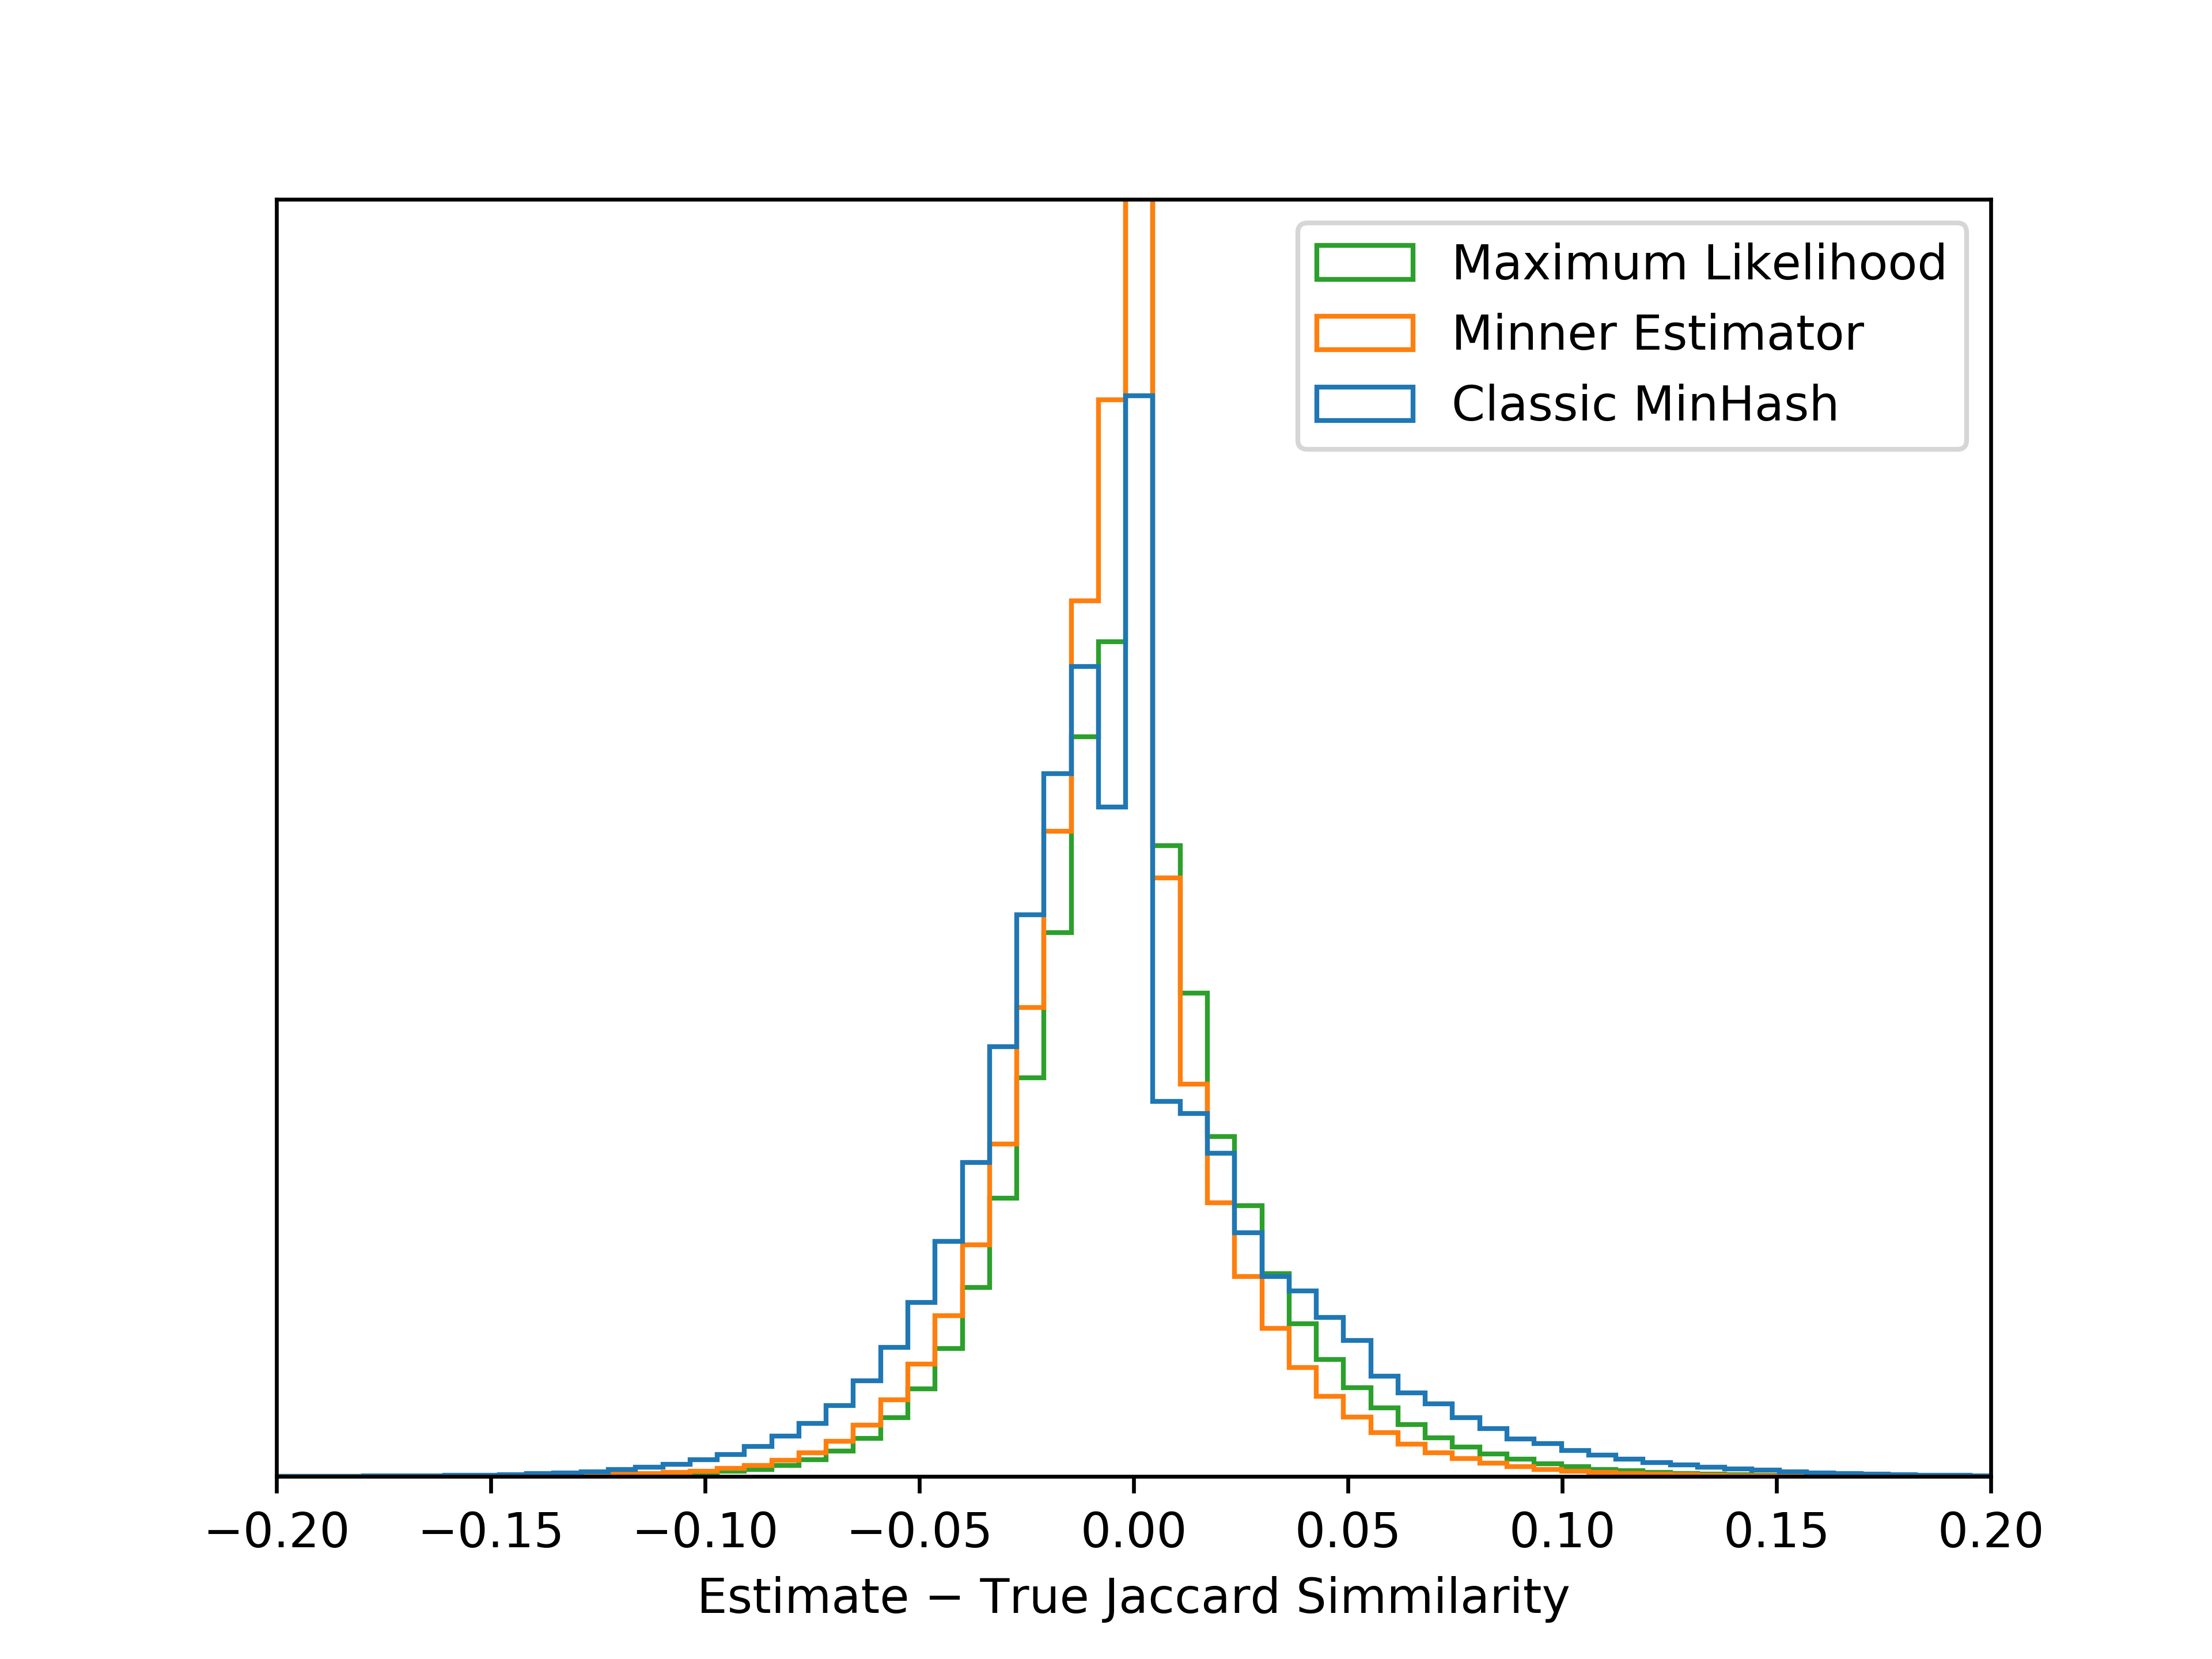
\includegraphics[trim=0 5 35 40,clip,width=\linewidth]{figures/hist2}
\caption{Density of estimation errors on Netflix dataset at $K=31$.
   %The empiric means are $0.0114$ for the symmetric estimator, 
%$0.0002$ for the fast estimator, and 
%$0.0038$ for the MLE estimator.
}
\end{figure}

\begin{figure}
   \centering
   % trim is left bottom right top
   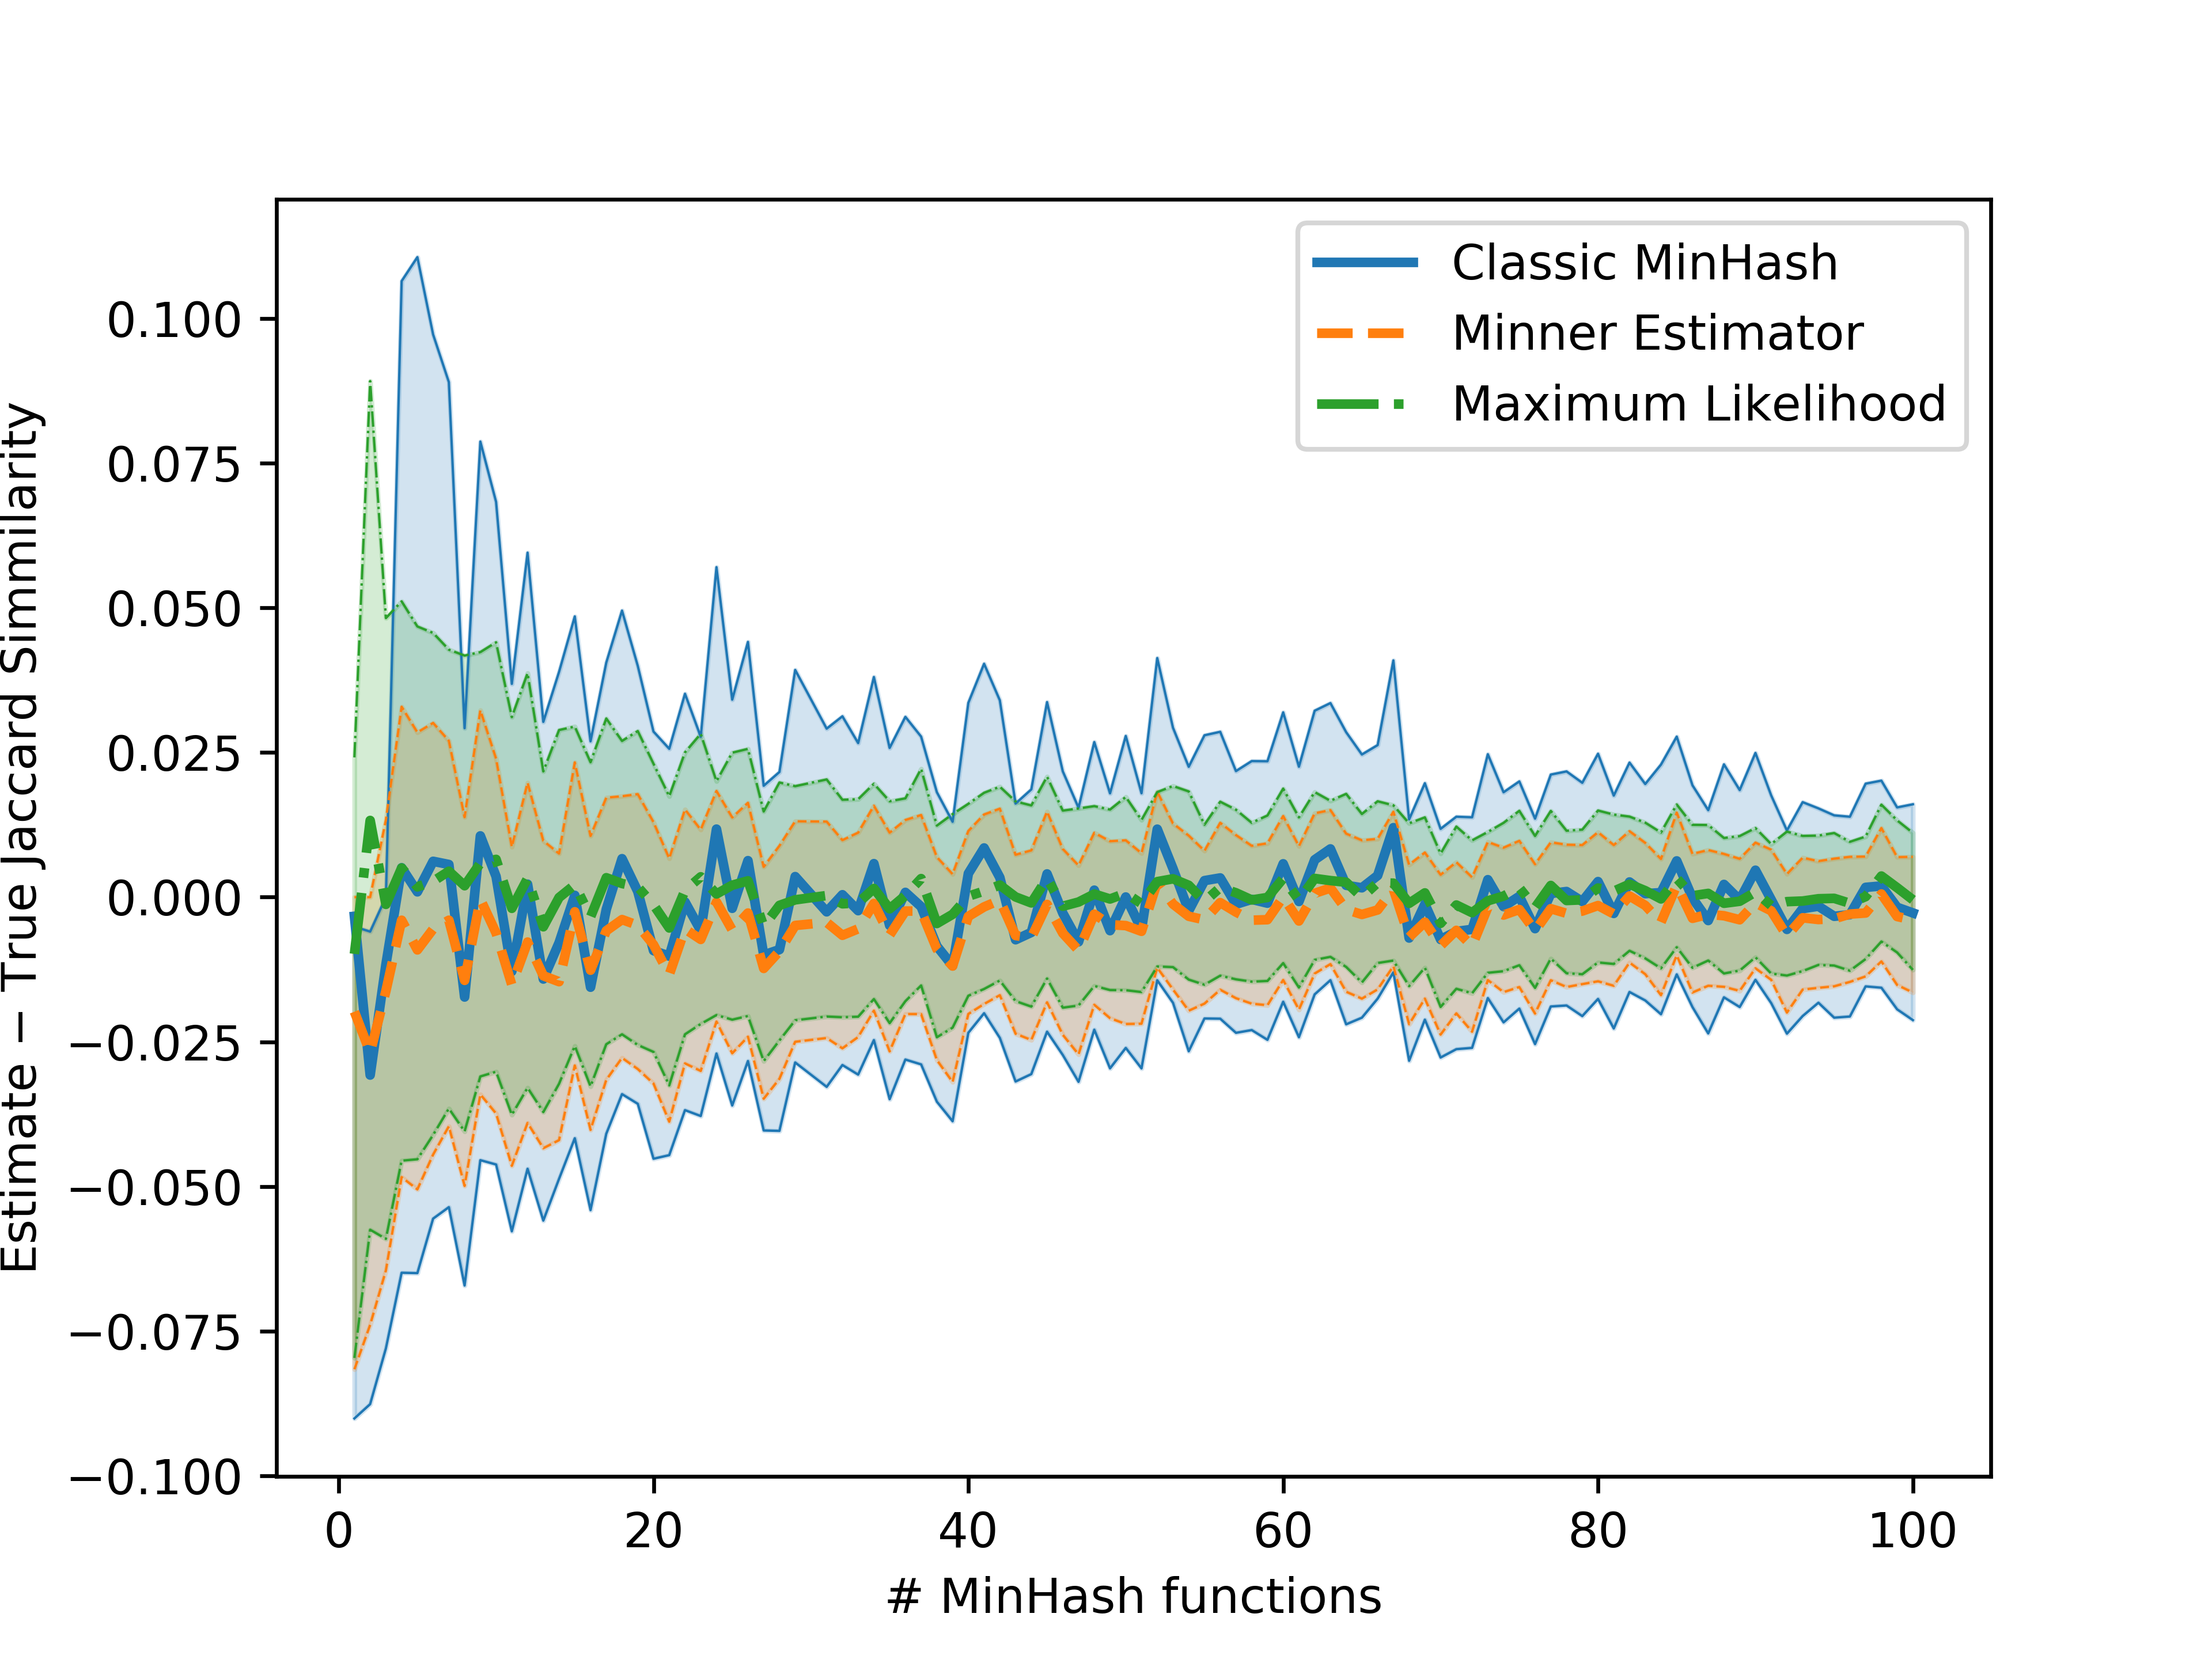
\includegraphics[trim=0 0 35 40,clip,width=\linewidth]{figures/var2}
   \caption{
      Mean values with 1 standard deviation bounds (15.9\% percentile)
      on the estimation error for 5 million pairs from the Netflix dataset.
   }
   \label{fig:var}
\end{figure}

%! TEX root = ../aminhash.tex

% Discuss results
% Explain conflicting results, unexpected findings and discrepancies with other research
% State limitations of the study
% State importance of findings

\section{Conclusion}

We have shown that it is possible to substantially improve upon the traditional MinHash estimator in the database or one-way communication setting.
Our analysis has shown one can reduce the global risk by nearly 30\%,
and much more when the size of the sets differ.
%The fact that our variance is $\frac{n_y}{n_x+n_y}$ of MinHash's variance suggests that our method might be particularly useful for containment queries, in which the 
Meanwhile, our experiments have shown a similar improvement in recall on standard datasets.

While our first estimator had a running time of $\Omega(K \min\{|X|,|Y|\})$, can be slow, we derived a faster $O(K)$ time estimator, which has a similar variance and often even an improved recall.
%The Minner estimator with newton=8 can sometimes give results quite different from MLE, because of the approximation into making it linear.
The success of our Minner estimator also suggests that the count of ``hash values smaller than the minimum'' could be used more widely.
Perhaps as part of the input supplied to Machine Learning pipelines working with coordinated sampling.

While our estimator only takes time $O(k)$ per data point, they do however still need to do at least two table lookups per value, where the classical estimator just needs to do a single equality comparison.
In \cref{sec:alg} we discussed how the table lookups could be done using fast SIMD instructions, as is done in the Product Quantization world, which presumably would close the remaining gap.
%Ideally our algorithm runtime should be dominated by loading data from memory into cache/registers.

\section{Open Problems}

Besides the SIMD considerations in \cref{sec:alg}, there are a number of potential future directions:
\begin{enumerate}
   \item Weighted MinHash~\cite{ioffe2010improved} And ``Probability MinHash''~\cite{moulton2018maximally} are common extensions of MinHash to non-binary data.
      As with classical MinHash all known estimators follow the symmetric paradigm, so could potentially see similar improvements to what we have shown in this paper.
%   \item Bottom-$k$ MinHash has often been shown to give better estimates than the $K$ independent hash functions MinHash we have studied.
%      Bottom-$k$ also has the benefit of faster hashing, which would translate to faster index generation time in the database setting.
%      The approach has nice combinatorial properties that might also lead to fast estimators.
   \item Is the Minner Estimator consistent? In \cref{sec:minner} we gave results that indicate Minner may not be unbiased.
      However, experimentally it appears to converge to the right value as $K\to\infty$.
   \item Use a Bayesian prior for $Y$.
      In \cref{sec:mle} we briefly discussed the possibility of assuming a prior on $Y$ other than the uniform distribution.
      Since all the datasets of Mann et al.~\cite{mann2016empirical} have some elements of the domain more common than others (and the Flickr dataset particularly so), such a prior, based on statistics on the dataset, could potentially be very efficient.
   \item Finally we suggest the task of finding the best possible sketch for sets in general.
      In~\cite{DBLP:conf/focs/AhleK20} it was shown that a best possible space partition exists for set similarity search with any set similarity measure.
      One could imagine a similar result, which would replace MinHash as the preferred quantization method for sets.
\end{enumerate}

% \begin{acks}
% Rasmus Pagh and Ninh Pahm
% \end{acks}


\begin{figure}
   %\hspace{-1em}
   \centering
   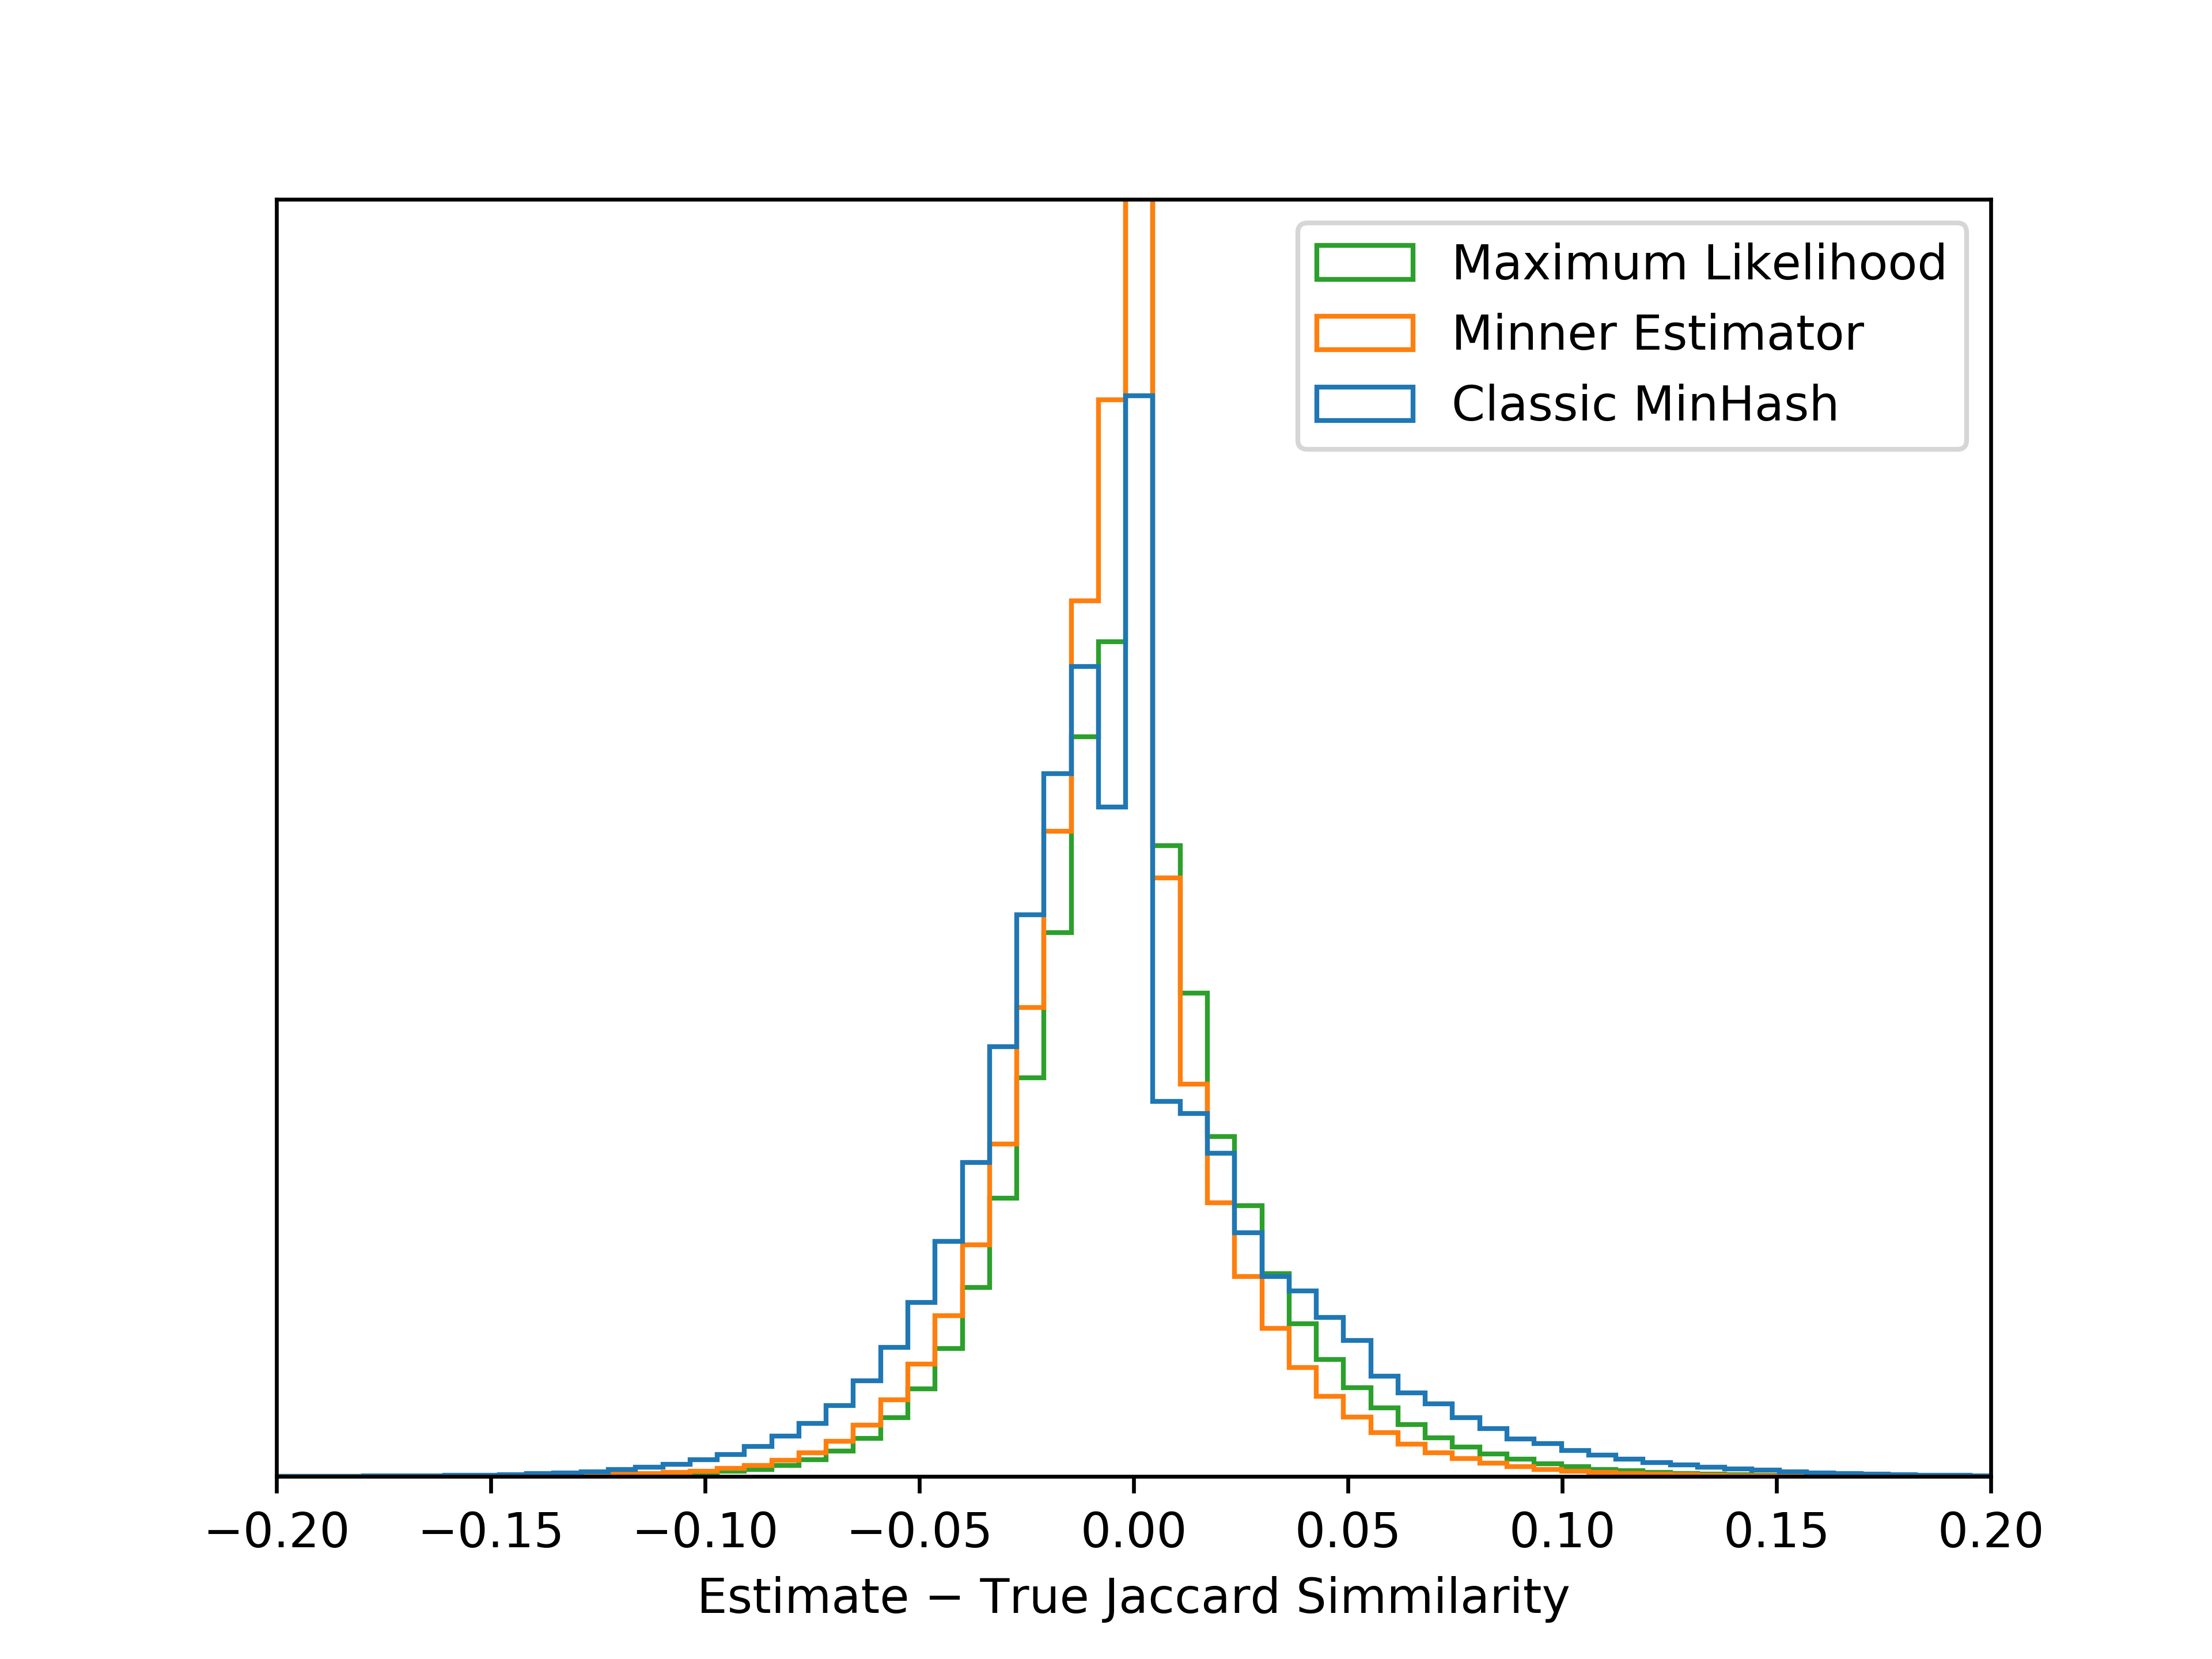
\includegraphics[trim=0 5 35 40,clip,width=\linewidth]{figures/hist2}
\caption{The density of estimation errors on Netflix dataset at $K=31$ over a million pairs.
%The empiric means are $0.0114$ for the symmetric estimator, 
%$0.0002$ for the Minner estimator, and 
%$0.0038$ for the Maximum likelihood estimator.
Besides a slightly better variation, the maximum likelihood estimator has a much better chance of getting a ``perfect'' estimate.
%The top of the plot has however been cut off so one can see the bottom more clearly.
}
\end{figure}



\bibliographystyle{ACM-Reference-Format}
\bibliography{minner}


%\appendix
%%! TEX root = ../aminhash.tex

\section{Appendix}

\subsection{Nice summation}
Let $n_x=|x|$ and $n_y=|y|$.
For a warm-up we show
\begin{align}
   \sum_{0\le m < u}
   \binom{n_x-k(m)-[m\in x]}{v-[m\in x]}
   \binom{u-m-[m\not\in x]-(n_x-k(m))}{n_y-v-[m\not\in x]}
   = \binom{n_x}{v}\binom{u-n_x}{n_y-v}
   .
\end{align}

We will use the following standard binomial sum:
\begin{align}
   \sum_{a<k<b}\binom{k}{c} &= \binom{b}{c+1} - \binom{a+1}{c+1}
   %\sum_{k=0}^u\binom{k}{c} &= \binom{b+1}{c+1} - \binom{a}{c+1}
\end{align}

Define a sequence $(a_i)_{i\in[0,n_x+1]}$ such that $a_0=-1$, $a_{i+1} = x_i$ for $i\in[n_x]$ and $a_{n_x+1}=u$,
where we see $x$ as a vector in $[u]^{n_x}$.

We consider the sum of terms for the chunk of $m$s between two consecutive $a$ values.
\begin{align}
   &
   %\sum_{0\le k \le n_x}
   \sum_{a_k < m < a_{k+1}}
   \binom{n_x-k}{v}
   \binom{u-m-1-(n_x-k)}{n_y-v-1}
   %+
   %\binom{n_x-k-1}{v-1}
   %\binom{u-a_{k+1}-(n_x-k)}{n_y-v}
   \\&=
   \binom{n_x-k}{v}
   \left[
   \binom{u-a_k-1-(n_x-k)}{n_y-v}
   -
   \binom{u-a_{k+1}-(n_x-k)}{n_y-v}
\right]
   \label{eq:sum_dif}
\end{align}
Define $c_k = \binom{u-a_k-(n_x-k+1)}{n_y-v}$,
We are the interested in the sum
\begin{align}
   \sum_{0\le k \le n_x}
   \binom{n_x-k}{v}(c_k-c_{k+1})
   +
   \sum_{0\le k < n_x}
   \binom{n_x-k-1}{v-1}c_{k+1}
   \label{eq:sum_all}
\end{align}
We substitute $k\mapsto k+1$ in the first term of \eqref{eq:sum_dif} to get the sum
\[
   \binom{n_x}{v}c_0
   +
   \sum_{0 < k+1 \le n_x}
   \binom{n_x-k}{v}
   c_k
   =
   \binom{n_x}{v}c_0
   +
   \sum_{0 \le k < n_x}
   \binom{n_x-k-1}{v}
   c_{k+1}
\]
which we can combine with the second term of \eqref{eq:sum_all}
using the fact that $\binom{n_x-k-1}{v} + \binom{n_x-k-1}{v-1} = \binom{n_x-k}{v}$
to give
\[
   \sum_{0\le k < n_x}
   \binom{n_x-k}{v}
   c_{k+1}
   .
\]
This allows cancellation with the second term of \eqref{eq:sum_dif},
leaving us with
\[
   \binom{n_x}{v}c_0
   -
   \binom{n_x-n_x}{v}c_{n_x+1}
   =
   \binom{n_x}{v}\binom{u+1-(n_x+1)}{n_y-v}
   -
   \binom{0}{v}
   \binom{0}{n_y-v}.
\]
Now $\binom{0}{v}=[v=0]$, so unless $n_y=0$ this second term is 0, leaving us with
$\binom{n_x}{v}\binom{u-n_x}{n_y-v}$.


\end{document}

